\documentclass[12pt,a4paper,oneside]{article}

\usepackage[spanish]{babel}
\addto\captionsspanish{\renewcommand{\tablename}{Tabla}}
\usepackage{caption} 

\usepackage[utf8]{inputenc}
\usepackage[T1]{fontenc}
\usepackage{mathpazo} 


\usepackage{csquotes}
\usepackage[dvipsnames]{xcolor}
\usepackage{graphicx}
\usepackage{booktabs}   
\usepackage{float}
\graphicspath{{../results/figures/}}
\newcommand{\tabla}[1]{\input{../results/tables/#1.tex}}

\usepackage{amsmath}
\usepackage{amsthm}

\theoremstyle{plain}
\newtheorem{proposicion}{Proposición}
\theoremstyle{definition}
\newtheorem{corolario}{Corolario}
\newtheorem{hipotesis}{Hipótesis}
\renewcommand\proofname{Demostración}

% hyperfootnotes=false evita que el \blfootnote de más abajo desincronice los
% anclajes de nota al pie de hyperref (pdfTeX: "Hfootnote.N ... does not exist").
\usepackage[hyperfootnotes=false]{hyperref}
\hypersetup{
    colorlinks=true,
    linkcolor=blue,
    citecolor=blue,
    urlcolor=blue
}
\usepackage{cleveref}

\AtBeginDocument{%
  \renewcommand{\crefpairconjunction}{ y }%
  \renewcommand{\creflastconjunction}{ y }%
  \renewcommand{\crefrangeconjunction}{ a }%
}

\crefname{table}{tabla}{tablas}
\Crefname{table}{Tabla}{Tablas}
\crefname{figure}{figura}{figuras}
\Crefname{figure}{Figura}{Figuras}
\crefname{section}{sección}{secciones}
\Crefname{section}{Sección}{Secciones}
\crefname{equation}{ecuación}{ecuaciones}
\Crefname{equation}{Ecuación}{Ecuaciones}
\crefname{proposicion}{proposición}{proposiciones}
\Crefname{proposicion}{Proposición}{Proposiciones}
\crefname{corolario}{corolario}{corolarios}
\Crefname{corolario}{Corolario}{Corolarios}
\crefname{hipotesis}{hipótesis}{hipótesis}
\Crefname{hipotesis}{Hipótesis}{Hipótesis}

% 1. Ajuste de márgenes (simétricos de 2.5cm)
\usepackage[
    margin=2.5cm,
    headsep=10mm,
    footskip=12mm
]{geometry}

% 2. Mayor interlineado
\usepackage{setspace}
\onehalfspacing % Puedes usar \doublespacing si requieres aún más espacio


\usepackage{titlesec}

% Formato para las secciones principales
\titleformat{\section}[block]
  {\normalfont\Large\bfseries\centering} % Centrado, fuente grande y negrita
  {\thesection.} % Agrega un punto después del número (ej. "1.")
  {0.8em} % Espacio entre el número y el título
  {}

\titleformat{\subsection}
  {\normalfont\large\bfseries}{\thesubsection}{0.8em}{}

% 3. Sin sangría y con separación entre párrafos
\usepackage{parskip}

% 4. Mejora de justificación automática
\usepackage{microtype}


\usepackage[backend=biber, style=apa]{biblatex}
\addbibresource{bibliografia.bib}

\makeatletter
\def\blfootnote{\xdef\@thefnmark{}\@footnotetext}
\makeatother

\title{\vspace{1.5cm}\textbf{Efecto de la entrada sobre la competencia local}\textsuperscript{*}}
\author{Joaquín Martínez\textsuperscript{\dag}}
\date{Borrador: Agosto, 2026}

\begin{document}

\maketitle

\blfootnote{\textsuperscript{*}Agradezco a Paola Bordón por su guía, apoyo y paciencia en este proceso. También quisiera agradecer a Alejandro Micco, Pablo Muñoz y Joaquín Hidalgo por la provechosa discusión alrededor de esta investigación. Cualquier error es mi responsabilidad.}
\blfootnote{\textsuperscript{\dag}Facultad de Economía y Negocios, Universidad de Chile. Correo: \href{mailto:joamartine@fen.uchile.cl}{\texttt{joamartine@fen.uchile.cl}}}

\renewcommand{\thefootnote}{\arabic{footnote}}
\setcounter{footnote}{0}

\begin{abstract}
\noindent
La sana competencia en el mercado minorista de combustible es crítica en el bienestar de los hogares y los costos de cadenas productivas. Este trabajo estima el efecto disciplinador sobre los precios que induce la entrada de una nueva estación de servicio en un mercado local. Utilizando bases de datos administrativas, oficiales y públicamente disponibles se aproximan los márgenes de venta e identifican entradas. Mediante un estudio de eventos se captura la respuesta en precios y márgenes frente a la entrada de un nuevo competidor en el mercado local. Se encuentra un efecto causal de alrededor del $4\%$ sobre los márgenes de venta en gasolina de 93 octanos y diesel a la vez que un efecto nulo en la gasolina de 97 octanos. La respuesta es mayor en estaciones que ex-ante presentan los mayores márgenes con respecto a su comuna. 
\end{abstract}

\vspace{0.5cm}
\noindent \textbf{Códigos JEL:} L13, L81, L11. \\
\noindent \textbf{Palabras clave:} Competencia local, Mercado de combustibles, Estudio de eventos. 


\renewcommand{\thefootnote}{\arabic{footnote}}
\setcounter{footnote}{0}



\newpage

\section{Introducción}

El precio del combustible tiene efectos sobre el bienestar social tanto por la asignación eficiente de los recursos mediante precios competitivos como por su incidencia en los costos de la cadena productiva. En Chile, los mecanismos institucionales determinan los costos de distribución minorista, y por ende los márgenes de venta son el componente principal por el cual se expresa la competencia entre estaciones de servicio (EDS). Medir y caracterizar la respuesta frente a un nuevo competidor orienta la política de competencia respecto al rol de las barreras de entrada.

El propósito de este estudio es investigar el efecto disciplinador inducido por un nuevo competidor en un mercado particularmente concentrado y con altas barreras de entrada. El informe de la \textcite{FNE2025informe} caracterizó el mercado de distribución minorista de combustible en Chile bajo una alta concentración e integración vertical en tres franquicias que controlan alrededor del $80\%$ de las EDS. El informe detalla que la regulación dentro de toda la cadena productiva elevan las barreras de entrada dificultando la presencia de nuevos competidores. Adicionalmente, el mercado es naturalmente de caracter geográfico, los márgenes de venta que una EDS de servicio puede imponer dependen no solo del número de competidores sino de la distancia entre ellos.

Considerando estas características, el mercado de combustible resulta interesante de investigar puesto que la alta visibilidad del precio y la perfecta homogeneidad del producto aislan el componente espacial como uno de los más importantes en la determinación del precio. Dado esto, el mercado de combustibles ha sido investigado bajo esta dimensión en múltiples trabajos, principalmente de corte transversal midiendo la densidad de competidores \parencite{CLEMENZGUGLER2006}. De manera estructural, \textcite{HOUDE2012} especifica los trayectos de los consumidores, y no su lugar de residencia, como las ubicaciones de un modelo de tipo Hotelling, de modo que la diferenciación espacial pasa a depender de la red vial y de la dirección de los flujos de tráfico. En Chile existen dos precedentes cercanos, ambos tesis de magíster de la Universidad de Chile: \textcite{CASTILLO2018} mide el efecto de la cercanía de estaciones rivales sobre el precio, distinguiendo entre redes integradas e independientes y construyendo distancias en tiempo de viaje entre todas las EDS georreferenciadas del país, y \textcite{SOLIS2025} documenta la dispersión de precios entre estaciones cercanas y la atribuye a costos de búsqueda del consumidor. En esta oportunidad se busca capturar el efecto promedio de una entrada sobre el precio de las incumbentes en un mercado local particular, siguiendo los métodos de \textcite{FISCHER2025, KOH2022}, que serán los articulos seminales de esta investgación. 

Una diferencia importante con respecto a estos articulos que justifica la exploración de este tema en Chile es que los mecanismos institucionales tales como el Mecanismo de Estabilización de Precios de los Combustibles (MEPCO) son públicos y de frecuencia semanal, al igual que los precios de paridad publicados por la Empresa Nacional del Petróleo (ENAP), lo que permite aproximar el costo mayorista que enfrentan las estaciones con información pública disponible.\footnote{\textcite{KOH2022} no observa márgenes y por tanto restringe su análisis a precios de venta y aproximaciones de márgenes que tienen una relevancia acotada. \textcite{FISCHER2025} compra la información de márgenes comercialmente. El MEPCO por lo tanto es útil en poder aproximar estos márgenes de venta con información pública} 

Como insumo para la investigación se explotan los datos históricos de las actualizaciones de precio de cada EDS junto a su localización y distribuidor. Adicionalmente, para aproximar el margen de venta de las estaciones se utilizan datos del precio mayorista de las estaciones considerando el MEPCO. Con el fin de falsear las hipótesis que se exponen más adelante se utiliza un estudio de eventos mediante un estimador de diferencias en diferencias con efectos fijos. El método encuentra efectos causales bajo el supuesto de exogeneidad del timing de entrada desde el punto de vista de la incumbente \parencite{ARCIDIACONO2020}, el cual se defiende más adelante.

Esta investigación aporta a la literatura en tres aspectos. El primero es de medición. \textcite{KOH2022} no observan el precio mayorista y deben restringir su análisis a los precios de venta, \textcite{FISCHER2025} acceden a márgenes a través de datos comerciales. El MEPCO permite aproximar el margen bruto de cada estación con información enteramente pública, y el trabajo documenta cómo hacerlo. 

El segundo aporte es testear mediante la estrategia empírica si los márgenes ex-ante de la entrada determinan el tamaño del efecto displicanador. Se encuentra que las estaciones que tienen márgenes mayores con respecto a su comuna son quienes más reducen sus precios ante la entrada de una competidora. 

El tercer aporte es reportar nueva evidencia causal sobre el comportamiento de las EDS frente a la entrada de nuevos competidores en una economía en desarrollo. Gracias a estas estimaciones tenemos más información para delimitar de manera más precisa los mercados locales en el mercado de combustibles chileno, relevante para un análisis de libre competencia. 

\input{sections/02_revision_literatura.tex}

\section{Descripción de la industria}

\subsection{Institucionalidad del sector}

\paragraph{La cadena productiva} La industria de los combustibles líquidos tiene cuatro etapas de producción: extracción, refinación, distribución mayorista y distribución minorista \parencite{FNE2025informe}. Siendo la distribución minorista la mitad de las ventas antuales de combustible del país. La ENAP es la única empresa que produce y refina petróleo crudo en Chile, insumo que es esencialmente importado siendo la producción nacional alrededor del $1\%$ con respecto a las importaciones. Si bien las grandes compañías mayoristas pueden abastecerse tanto de las refinerías de ENAP como importar directamente, las empresas de menor tamaño se abastecen únicamente de ENAP \parencite{FNE2025informe}.\footnote{El $12\%$ de la oferta nacional de gasolinas y el $73\%$ del diésel son importados} La consecuencia relevante para este trabajo es que el costo de adquisición de las EDS está anclado, para la generalidad del mercado, a una referencia única.

En términos de producto, las gasolinas de 93, 95 y 97 octanos y el petróleo diésel constituyen el objeto de análisis. El diésel explica algo más de la mitad de las ventas nacionales de combustibles líquidos, aunque con usos diversos en la industria, el comercio y el transporte, las gasolinas, que son consumidas casi exclusivamente por el transporte terrestre, representan en conjunto alrededor de un tercio, con la de 93 octanos como la de mayor peso \parencite{FNE2025informe}.

\paragraph{El costo mayorista y el MEPCO} El precio mayorista que enfrentan los distribuidores se construye sobre el precio de paridad de importación que fija semanalmente el Ministerio de Energía, previo informe de la Comisión Nacional de Energía (CNE), y sobre él operan los impuestos específicos de la ley N°18.502.

La ley N°20.765 de 2014 creó el Mecanismo de Estabilización de Precios de los Combustibles (MEPCO), que atenúa la transmisión de las variaciones internacionales al precio interno \parencite{LEY20765}.\footnote{El mecanismo opera a través de un componente variable que se suma o se resta al componente base del impuesto específico. Su regla de cálculo es explícita: se proyecta un ``precio base'' como, el precio que ENAP informará la semana siguiente suponiendo un componente variable nulo, incluidos IVA e impuesto específico base, y se lo compara con el precio efectivamente informado la semana anterior. Cuando la diferencia excede el $0{,}8\%$ del promedio de las dos últimas semanas del precio base de la gasolina de 93 octanos, el componente variable se ajusta para absorber el exceso.}  En la práctica, el mecanismo acota la variación semanal del precio mayorista en torno a un umbral con el objetivo de estabilizar el precio final.

Tres rasgos del MEPCO son importantes para la estrategia empírica. Primero, es una referencia nacional, el precio de paridad se fija una vez por semana y entra en vigencia el jueves siguiente, sin diferenciación geográfica. Segundo, es una referencia fijada por regla y publicada, no negociada bilateralmente, por lo que no puede responder a condiciones de competencia locales. Tercero, la propia ley precisa que los precios de referencia y de paridad ``serán mera referencia y no constituirán precios mínimos ni máximos de venta'' \parencite{LEY20765}. Es decir, el MEPCO regula el costo mayorista, no el precio minorista, que las EDS fijan libremente. Es esta combinación la que permite aproximar el margen de cada estación e identificar en él el componente competitivo del precio.

\paragraph{Estructura del mercado minorista} La distribución minorista está dominada por tres compañías integradas verticalmente. Al año 2023, Copec concentraba el $39\%$ de las EDS del país, Petrobras el $21\%$ y Shell el $16\%$, el $24\%$ restante corresponde a distribuidoras de bandera blanca, esto es, estaciones que operan bajo marca propia o sin marca, con redes reducidas, menores costos operativos y menores estándares de servicio \parencite{FNE2025informe}.

La integración vertical no siempre implica propiedad. Las mayoristas participan en el mercado minorista mediante redes de EDS propias o de terceros, y la relación contractual admite dos formas que difieren en un punto decisivo para este análisis. Bajo el modelo de consignación, el combustible sigue siendo propiedad de la mayorista, que determina el precio de venta al público, y la administradora de la EDS recibe como remuneración un margen por litro vendido. Bajo el modelo de concesión, en cambio, la administradora compra previamente el combustible y es ella quien fija el precio al público \parencite{FNE2025informe}. La coexistencia de ambos regímenes implica que una fracción no menor de las decisiones de precio observadas en los datos se toma a nivel de cadena y no de estación, lo que motiva incorporar efectos fijos de distribuidor interactuados con el tiempo en las especificaciones empíricas.

\paragraph{Homogeneidad del producto y transparencia de precios} Dos rasgos regulatorios definen el tipo de competencia posible en este mercado. El primero es la homogeneidad, los combustibles deben cumplir especificaciones de calidad fijadas por el Ministerio de Energía, de modo que dos productos del mismo octanaje son sustitutos perfectos con independencia de la marca que los comercialice \parencite{FNE2025informe}. El segundo es la transparencia. Desde 2012 la CNE administra la plataforma Bencina en Línea, y las EDS están obligadas
por norma a informar sus precios de venta cada vez que éstos varían, obligación sujeta a fiscalización y multas.

\paragraph{El carácter local de la competencia} La FNE ha definido de manera consistente el mercado relevante de producto como la distribución minorista de combustibles líquidos a través de EDS, segmentable según tipo de combustible. Respecto del mercado geográfico, ha sostenido que en el caso de las estaciones de servicio éste es \textcquote{FNE2021informe}{%
eminentemente local, con una ampliación del área geográfica de competencia a través de cadenas de sustitución, cuyo efecto se disipa en la medida que la distancia es mayor, por lo que existiría un punto en que la presión competitiva de una estación de servicio determinada sobre la otra deja de ser relevante}.
En la práctica ha considerado radios de tres a cinco kilómetros, sin descartar radios menores.

\paragraph{Barreras a la entrada} Tanto la FNE como el Tribunal de Defensa de la Libre Competencia han constatado en repetidas ocasiones la existencia de barreras a la entrada en este mercado. Éstas se refieren principalmente a la escasez de terrenos aptos para la instalación o arriendo de estaciones de servicio, dadas las exigencias de los planos reguladores en las zonas urbanas más saturadas, que son al mismo tiempo las de mayor atractivo comercial \parencite{FNE2021informe}. A ello se suman la regulación sectorial a lo largo de toda la cadena productiva, que involucra a distintas autoridades, y la inversión en infraestructura que requiere un potencial entrante \parencite{FNE2025informe}.

\subsection{Modelo de competencia espacial}

El marco natural para este mercado es el modelo de ciudad circular de \textcite{SALOP1979}.\footnote{El modelo de \textcite{SALOP1979} es una variante del de \textcite{HOTELLING1929}, del que hereda todo lo que esta aplicación necesita: consumidores distribuidos uniformemente sobre un espacio, demanda unitaria e inelástica, un costo de desplazamiento $c$ por unidad de distancia y ninguna preferencia entre vendedores que no sea el precio más el costo de llegar hasta ellos. Se prefiere la versión circular porque la recta de \textcite{HOTELLING1929} tiene extremos y, con ellos, posiciones asimétricas que impiden un equilibrio simétrico con más de dos firmas. La circunferencia elimina ese problema y permite obtener el resultado en el número de competidoras, $p = m + c/n$, que es justamente la estática comparativa que este trabajo contrasta.} Los combustibles son un bien homogéneo, los precios son observables y la regulación impide diferenciación relevante en el producto, de modo que la única fuente sustantiva de diferenciación es la ubicación. Un consumidor prefiere la EDS más cercana salvo que otra compense la distancia con un precio menor. Esta subsección recoge únicamente lo indispensable para plantear las hipótesis. Los resultados no son una adaptación del modelo sino el modelo mismo, y el Anexo~\ref{anexo:modelo} los desarrolla, indica la ecuación y la página de \textcite{SALOP1979} de las que proviene cada uno y discute las limitaciones del marco.

El mercado local de una estación se representa por una circunferencia de perímetro unitario sobre la que se distribuyen uniformemente $L$ consumidores de demanda unitaria y operan $n$ EDS equiespaciadas, de modo que la distancia entre dos contiguas es $1/n$. Un consumidor que se desplaza una distancia $x$ incurre en un costo $cx$, con $c>0$. Cada estación enfrenta un costo fijo $F$ y un costo marginal $m$ que, por ser el MEPCO una referencia nacional, es común a todas ellas en una fecha dada.\footnote{Si bien los costos mayoristas sí difieren en la realidad entre estaciones, se hace este supuesto de igual costo mayorista tanto para el modelo teórico como para la parte empírica.} El margen bruto
\begin{equation}
    \mu_i \equiv p_i - m
    \label{eq:def-margen}
\end{equation}
recoge entonces toda la variación de precios entre estaciones en un mismo instante y es, entendido así, el componente competitivo del precio. Como el número de competidoras dentro del radio en que la sustitución es efectiva difiere entre estaciones de una misma comuna, cada EDS enfrenta su propio $n_i$, y es esa variación la que el modelo traduce en variación de márgenes.

\begin{proposicion}[Margen de equilibrio]
\label{prop:margen}
En el equilibrio de Nash en precios de la región competitiva, con $n$ estaciones
equiespaciadas,
\begin{equation}
    \mu = \frac{c}{n} .
    \label{eq:margen}
\end{equation}
\end{proposicion}

\begin{corolario}[Efecto de una entrada]
\label{cor:entrada}
La llegada de una competidora al mercado local de la incumbente altera su margen
de equilibrio en
\begin{equation}
    \Delta\mu = \frac{c}{n+1} - \frac{c}{n} = -\,\frac{c}{n(n+1)} \;<\; 0 ,
    \label{eq:efecto}
\end{equation}
y, dado que $m$ no se altera, el precio cae en la misma magnitud.
\end{corolario}

\paragraph{Hipótesis contrastables} De \eqref{eq:margen} y \eqref{eq:efecto} se desprenden las tres hipótesis que la estrategia empírica somete a prueba.

\begin{hipotesis}[Efecto disciplinador]
\label{hip:nivel}
La entrada de un competidor reduce el precio y el margen de las incumbentes del
mercado local.
\end{hipotesis}
El signo de \eqref{eq:efecto} es inequívoco, y el efecto es permanente porque opera sobre el equilibrio y no sobre una desviación transitoria.

\begin{hipotesis}[Atenuación espacial]
\label{hip:distancia}
El efecto decrece en magnitud con la distancia entre la entrante y la incumbente, y se anula a partir de un umbral.
\end{hipotesis}
Si la entrante queda fuera del radio en que la sustitución es efectiva, la incumbente sigue enfrentando el mismo $n_i$ y el efecto es exactamente nulo. La predicción a nivel de estación es entonces discontinua; el perfil suave que se estima por anillos de distancia resulta de promediar ese umbral sobre estaciones con radios de mercado distintos.

\begin{hipotesis}[Heterogeneidad por margen previo]
\label{hip:margen}
El efecto es mayor sobre las incumbentes cuyo margen previo a la entrada era más alto en relación con su mercado local.
\end{hipotesis}
Por \eqref{eq:margen} el margen es un estadístico suficiente del aislamiento espacial de la estación. Invirtiendo esa expresión como $n = c/\mu$ y sustituyéndola en \eqref{eq:efecto} se obtiene $|\Delta\mu| = \mu^{2}/(c+\mu)$, creciente en el margen previo tanto en niveles como en términos relativos.


\section{Estrategia Empírica}

\subsection{Datos}

\paragraph{Fuentes}

La investigación combina dos fuentes, todas de acceso público. La primera es el registro histórico de precios de la Comisión Nacional de Energía (CNE). Cada observación corresponde a una actualización de precio informada por una EDS para un combustible determinado, con su fecha, y viene acompañada de la identificación de la estación, su distribuidor, sus coordenadas geográficas y su comuna y región. Como las EDS están obligadas por norma a informar cada variación de precio, el registro constituye un censo de la evolución de precios del mercado y no una muestra. La serie utilizada cubre desde enero de 2012 hasta julio de 2026.\footnote{Adicionalmente la CNE dispone información de servicios complementarios que ofrece cada EDS: tienda de conveniencia, lavado, baño público, farmacia, surtidor de camiones, entre otros. Estos atributos se emplean únicamente con fines descriptivos y de balance, ya que solo se dispone de la última actualización de cada estación y no de su evolución en el tiempo.}

La segunda es la serie semanal del precio mayorista con MEPCO, publicada por el Ministerio de Hacienda. Cubre desde el 7 de agosto de 2014 hasta el 2 de julio de 2026 y consta de 622 semanas consecutivas sin interrupciones, todas con vigencia a partir del día jueves, tal como establece la ley \parencite{LEY20765}. La serie está disponible para las gasolinas de 93 y 97 octanos y para el diésel, no existe una referencia MEPCO para la gasolina de 95 octanos, que por ello queda fuera de todo análisis de márgenes.

\paragraph{Construcción del panel}

El registro de la CNE genera una fila cada vez que una estación informa un precio, de modo que las observaciones son irregulares en el tiempo y no constituyen un panel. Su transformación en un panel balanceado descansa en tres decisiones, cuyo detalle e implementación se documentan en el Anexo~\ref{anexo:datos}. La unidad de análisis es la estación física y no el identificador administrativo, porque un mismo local puede aparecer en el registro bajo más de un código. Los identificadores que corresponden a un mismo local se fusionan en una sola unidad, de no hacerlo, un cambio de operador se contaría como una salida seguida de una entrada, y un registro duplicado inflaría el conteo de competidores cercanos.

El panel se construye a frecuencia semanal sobre la grilla de jueves del MEPCO, y de ahí se colapsa a frecuencia mensual. La semana no es una elección arbitraria, es la cadencia efectiva con que las estaciones reportan y es también la frecuencia nativa del precio mayorista. En esa grilla, el $81{,}1\%$ de las celdas corresponde a un precio efectivamente informado esa semana y el resto a un precio vigente arrastrado desde el último reporte, con un tope que impide arrastrarlo a través de períodos en que la estación no operaba. El margen bruto se define como el precio de venta menos el precio mayorista con MEPCO vigente esa semana, conforme a la \Cref{prop:margen}. Al ser el MEPCO una referencia nacional, el costo se adjudica por combustible y semana, no por estación.

El resultado es un panel semanal de 4.663.553 observaciones sobre 2.030 estaciones y 758 semanas, y su colapso mensual de 283.695 observaciones sobre 175 meses.

\paragraph{Definición de los eventos y de los grupos de comparación} Una entrada se define como el primer mes en que una estación física aparece en el registro, sujeto a tres restricciones que determinan qué eventos pueden usarse como tratamiento y que el Anexo~\ref{anexo:datos} detalla. Con estas restricciones, una incumbente se clasifica como tratada si experimenta una entrada dentro de un radio de 2 kilómetros mientras ya está operando. Las restantes conforman el grupo de comparación y se subdividen en un anillo, entre 2 y 5 kilómetros del evento más cercano, y un grupo lejano, a más de 5 kilómetros de toda entrada. La \Cref{tab:resumen} resume la composición resultante de la muestra.\footnote{Las salidas requieren una advertencia. El cambio de régimen de reporte de la CNE entre los archivos antiguos y los actuales deja una cicatriz en los datos que impide fechar con confianza el cierre de una estación en torno al quiebre, el Anexo~\ref{anexo:datos} documenta su origen y su magnitud. La limitación no afecta al diseño, que se construye exclusivamente sobre entradas.}

\begin{table}[H]
\centering
\caption{Composición de la muestra}
\label{tab:resumen}
\tabla{tab_desc_resumen}
\end{table}

La tabla y las figuras que siguen tienen por objeto mostrar que el panel reúne las condiciones que el diseño de identificación requiere, tales como número suficiente de eventos, dispersos en el tiempo, con grupos de comparación bien poblados y con variables de resultado que se comportan de manera estable.

La \Cref{fig:entradas} presenta las entradas por año y por marca de la estación entrante, desde 2014, que es el período en que rige el MEPCO y del que provienen las cohortes de tratamiento. Los eventos se distribuyen a lo largo de toda la serie. Destaca que la bandera blanca es el principal entrante del mercado, con 184 de las 482 entradas, por sobre Copec con 140.

\begin{figure}[H]
\centering
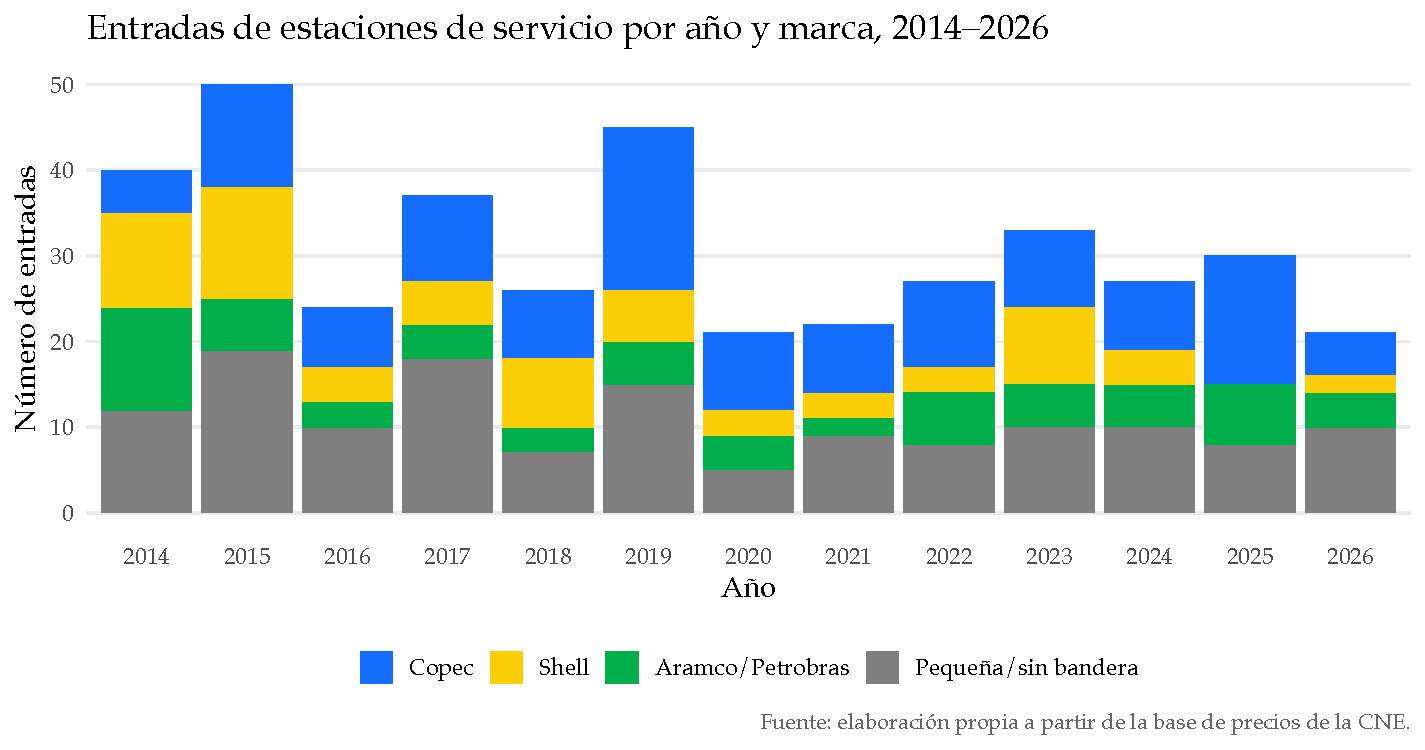
\includegraphics[width=\textwidth]{desc_entradas_por_anio.pdf}
\caption{Entradas por año y marca de la estación entrante}
\label{fig:entradas}
\end{figure}

La \Cref{fig:precio} muestra la evolución del precio promedio nacional por combustible. Las cuatro series se mueven juntas y están dominadas por el costo mayorista, que es común a todas las estaciones: es precisamente esa componente la que el margen descuenta. La \Cref{fig:margen} presenta el margen bruto promedio a partir de agosto de 2014. A diferencia del precio, el margen se mueve en un rango acotado, lo que confirma que descontar el MEPCO aísla una variable de nivel comparable a lo largo del tiempo y no una tendencia macroeconómica.

\begin{figure}[H]
\centering
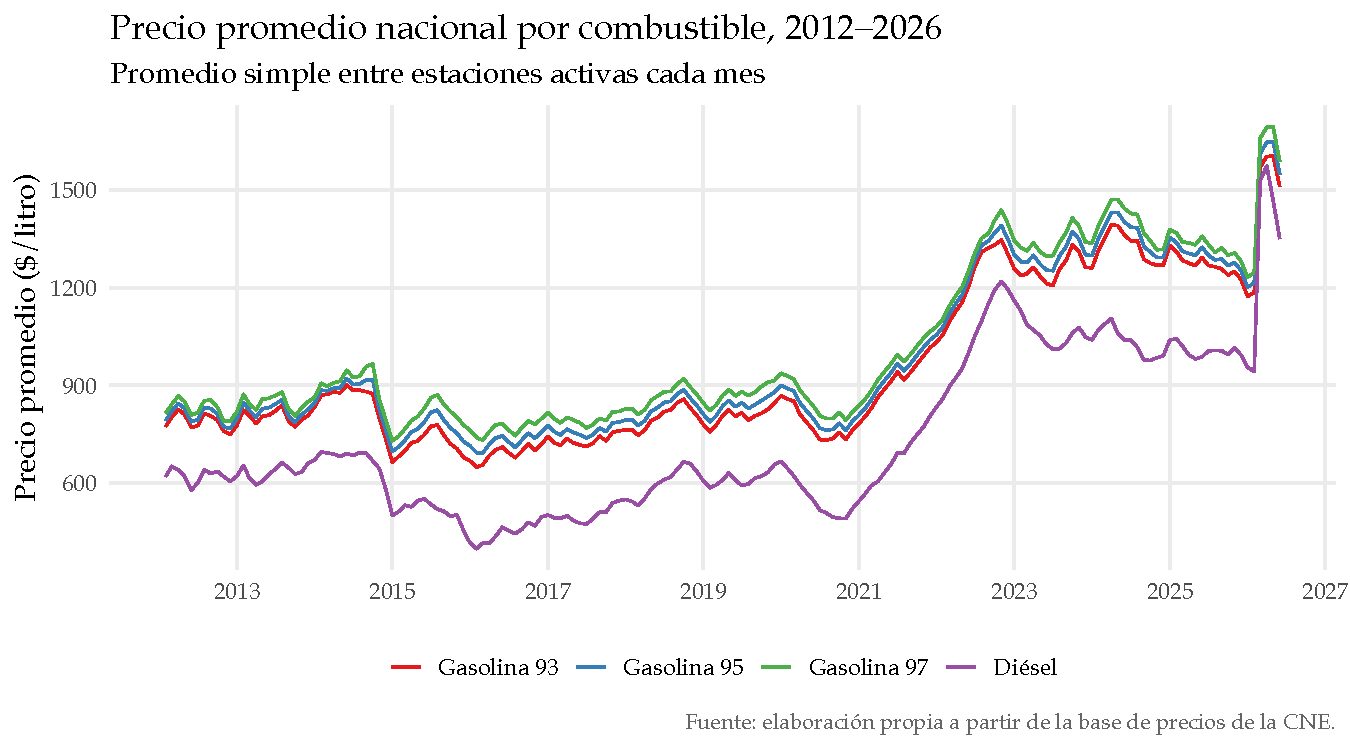
\includegraphics[width=0.9\textwidth]{desc_precio_promedio.pdf}
\caption{Precio promedio nacional por combustible}
\label{fig:precio}
\end{figure}

\begin{figure}[H]
\centering
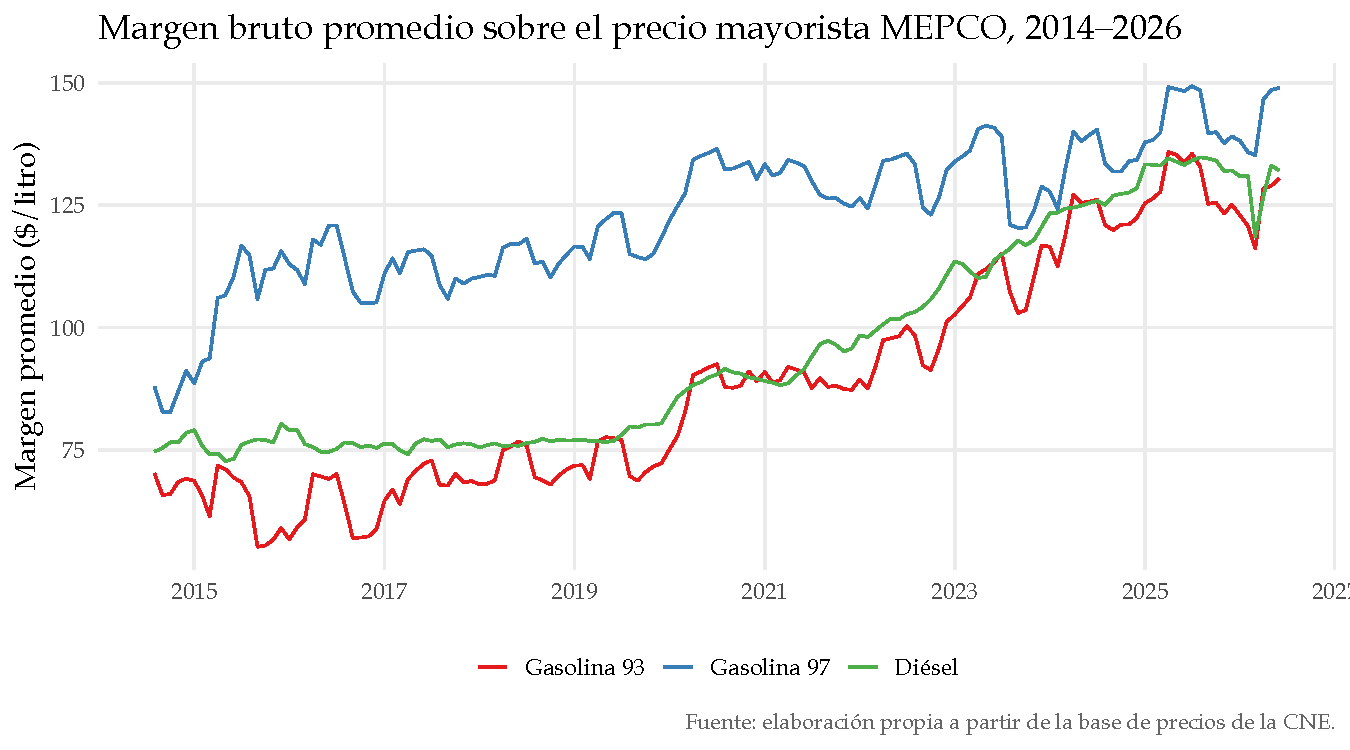
\includegraphics[width=0.9\textwidth]{desc_margen_promedio.pdf}
\caption{Margen bruto promedio sobre el precio mayorista con MEPCO}
\label{fig:margen}
\end{figure}

Por último, la \Cref{fig:mercado} describe el mercado local en el momento en que ocurre cada entrada. El $72{,}6\%$ de las entradas tiene al menos una estación vecina dentro de 2 kilómetros, con un promedio de 3,4 vecinos y una mediana de 2. Dos rasgos importan para la interpretación. Primero, los mercados afectados son efectivamente locales y poblados, de modo que la entrada constituye un cambio apreciable en la estructura competitiva y no una perturbación marginal. Segundo, solo el $19\%$ de las estaciones vecinas comparte marca con la entrante, lo que indica que la entrada típica es la llegada de un competidor y no la expansión de la red de una misma cadena.

\begin{figure}[H]
\centering
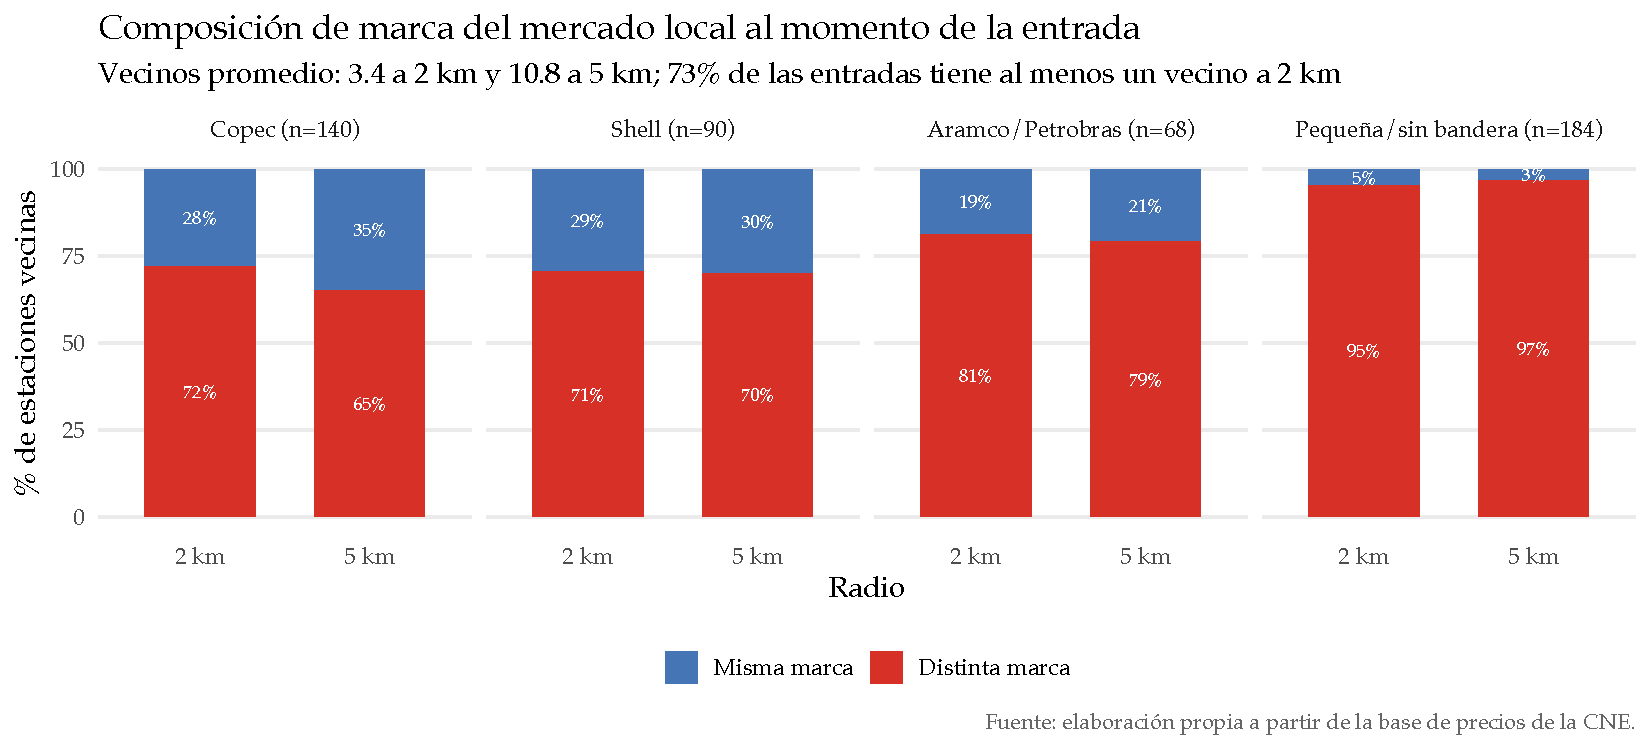
\includegraphics[width=\textwidth]{desc_mercado_local.pdf}
\caption{Composición de marca del mercado local al momento de la entrada}
\label{fig:mercado}
\end{figure}

\subsection{Identificación}

La estrategia sigue de cerca a \textcite{FISCHER2025}, cuyo objeto de estudio el efecto de la entrada de una estación sobre los precios de las incumbentes de su mercado local es el mismo de este trabajo. Se estima un estudio de eventos sobre el panel mensual de estaciones,
%
\begin{equation}
    y_{it} = \alpha_i + \lambda_t + \gamma_{r(i)a(t)} + \delta_{m(i)a(t)}
             + \sum_{\substack{\tau=-4 \\ \tau \neq -1}}^{4}
               \beta_\tau \, D^{\tau}_{it} + \varepsilon_{it},
    \label{eq:es}
\end{equation}
%
donde $y_{it}$ es el precio en logaritmo o el margen de la estación $i$ en el mes $t$, $\alpha_i$ es un efecto fijo de estación; $\lambda_t$ uno de mes, $\gamma_{r(i)a(t)}$ uno de región por año y $\delta_{m(i)a(t)}$ uno de marca por año. El indicador $D^{\tau}_{it}$ vale uno si la estación $i$ es tratada y el mes $t$ cae en el $\tau$-ésimo bin de seis meses respecto de la entrada que la trata. Los bins se agrupan en los extremos, de modo que $\tau \le -4$ y $\tau \ge 4$ acumulan todo lo que ocurre más allá de la ventana, y $\tau = -1$ es la categoría omitida. La ventana de cuatro bins previos y cinco posteriores, así como el agrupamiento de los extremos, replican el formato de reporte de \textcite{FISCHER2025}. Los errores estándar se agrupan a nivel de comuna.

El efecto promedio se obtiene de la versión estática de \eqref{eq:es},
%
\begin{equation}
    y_{it} = \alpha_i + \lambda_t + \gamma_{r(i)a(t)} + \delta_{m(i)a(t)}
             + \beta \, \mathrm{Post}_{it} + \varepsilon_{it},
    \label{eq:did}
\end{equation}
%
donde $\mathrm{Post}_{it}$ vale uno para una estación tratada desde el mes de la entrada en adelante.

Ambas especificaciones se estiman por efectos fijos bidireccionales sobre un diseño de adopción escalonada, situación en la que el estimador es un promedio ponderado de comparaciones entre cohortes que puede recibir ponderaciones negativas cuando el efecto del tratamiento varía entre ellas \parencite{CALLAWAYSANTANNA2021, SUNABRAHAM2021, DECHAISEMARTIN2020, BORUSYAK2024}. El Anexo~\ref{anexo:robustez} reestima el efecto promedio con el estimador de \textcite{SUNABRAHAM2021}, que nunca emplea como control a una incumbente ya tratada, y obtiene el mismo resultado; es la misma verificación que realizan \textcite{FISCHER2025} sobre su propio diseño.

Dos elementos de \eqref{eq:es} merecen justificación. El efecto fijo de estación absorbe todo atributo invariante del local tales como su ubicación, tamaño, y posición relativa dentro del mercado local, de modo que la identificación proviene únicament  de la variación dentro de cada estación. El efecto fijo de marca por año, que \textcite{FISCHER2025} no incorpora, responde a un rasgo propio del caso
chileno documentado en la sección anterior.\footnote{Bajo el modelo de consignación el precio de venta al público lo determina la compañía mayorista, y con tres cadenas que concentran cerca del $80\%$ de las EDS, un movimiento nacional de cualquiera de ellas es un confusor que ni el efecto fijo de estación ni el de región por año absorben.}

El supuesto de identificación es que el momento en que la entrada se materializa es exógeno desde la perspectiva de la incumbente, condicional en los efectos fijos de \eqref{eq:es}. Es el supuesto de \textcite{ARCIDIACONO2020}, adoptado también por \textcite{FISCHER2025} y por \textcite{KOH2022}. No exige que la ubicación de la entrada sea exógena (de hecho, no lo es) sino solo que, dado que una entrada va a ocurrir en un mercado, la fecha precisa  en que ocurre no responda a la evolución de los precios de las incumbentes. Este supuesto se defiende por las regulaciones que conlleva abrir una nueva estación y se justifica empíricamente más adelante.

\textcite{FISCHER2025} comparan las incumbentes tratadas contra el conjunto de estaciones no tratadas, sin construir un anillo de control. Este trabajo adopta el mismo criterio, y la \Cref{tab:control} justifica la elección estimando \eqref{eq:did} bajo las tres definiciones posibles del grupo de comparación: el anillo de estaciones entre 2 y 5 kilómetros del evento, las estaciones lejanas a más de 5 kilómetros de toda entrada, y la unión de ambas, que es el conjunto de las nunca tratadas.

\subsubsection{Efectos sobre precios y márgenes}

\begin{table}[H]
\centering
\caption{Efecto de la entrada sobre el precio, según el grupo de comparación}
\label{tab:control}
\tabla{tab_att_control}
\end{table}

Las tres definiciones de control entregan básicamente el mismo resultado. Para elegir el grupo de control hay que considerar dos criterios: el número de estaciones de control y la ausencia de spillovers, esto es, que ninguna estación del grupo de comparación esté ella misma expuesta al efecto de la entrada. El segundo criterio importa porque, como muestra \textcite{BUTTS2023}, cuando el control está parcialmente expuesto al tratamiento el estimador de diferencias en diferencias deja de recuperar el efecto de interés; en este caso la exposición del control tiene el mismo signo que el efecto sobre las tratadas, de modo que el sesgo atenúa la estimación hacia cero. Por lo que tanto controles lejanos como nunca-tratadas sirven, se elige nunca-tratadas. El Anexo~\ref{anexo:control} desarrolla esta comparación con el balance de covariables y los tests de tendencias previas de cada grupo.

La \Cref{fig:es} presenta el estudio de eventos de \eqref{eq:es} bajo la
especificación principal. Las trayectorias son planas antes de la entrada y caen de manera abrupta en el bin de la entrada, sin revertirse en los cinco bins posteriores, es decir, a lo largo de dos años y medio. La persistencia importa, un efecto que se disipara sería compatible con una reacción transitoria de posicionamiento, mientras que uno persistente indica un cambio en el equilibrio del mercado local, que es lo que predice el \Cref{cor:entrada}.

\begin{figure}[H]
\centering
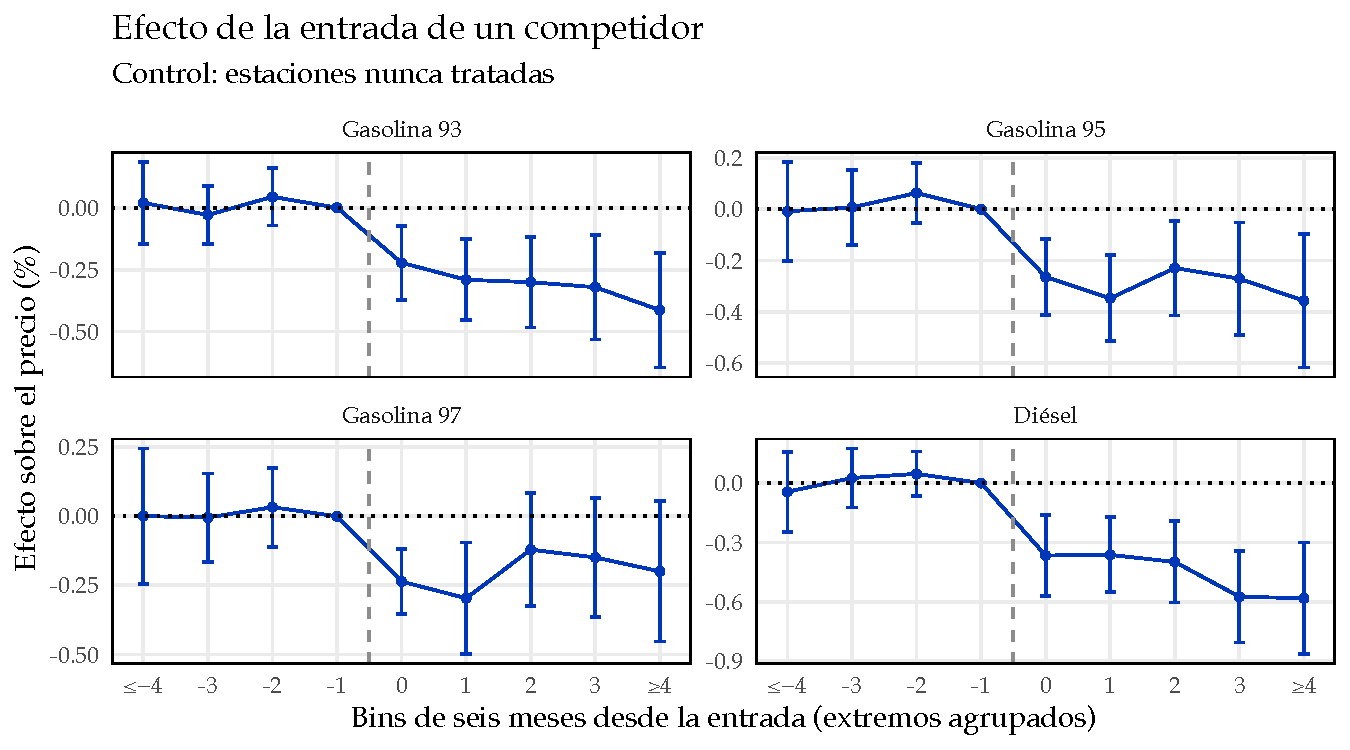
\includegraphics[width=\textwidth]{es_control_nunca.pdf}
\caption{Efecto de la entrada sobre el precio de las incumbentes}
\label{fig:es}
\end{figure}
La \Cref{fig:ff} presenta el efecto sobre el margen para los bienes disponibles en las bases del MEPCO, con las dos definiciones de mercado local como series. Las dos filas son el mismo objeto en unidades distintas: la superior expresa el efecto en pesos por litro y la inferior como porcentaje del margen previo, de modo que la primera indica cuánto cae el margen y la segunda qué fracción de él se pierde.

\begin{figure}[H]
\centering
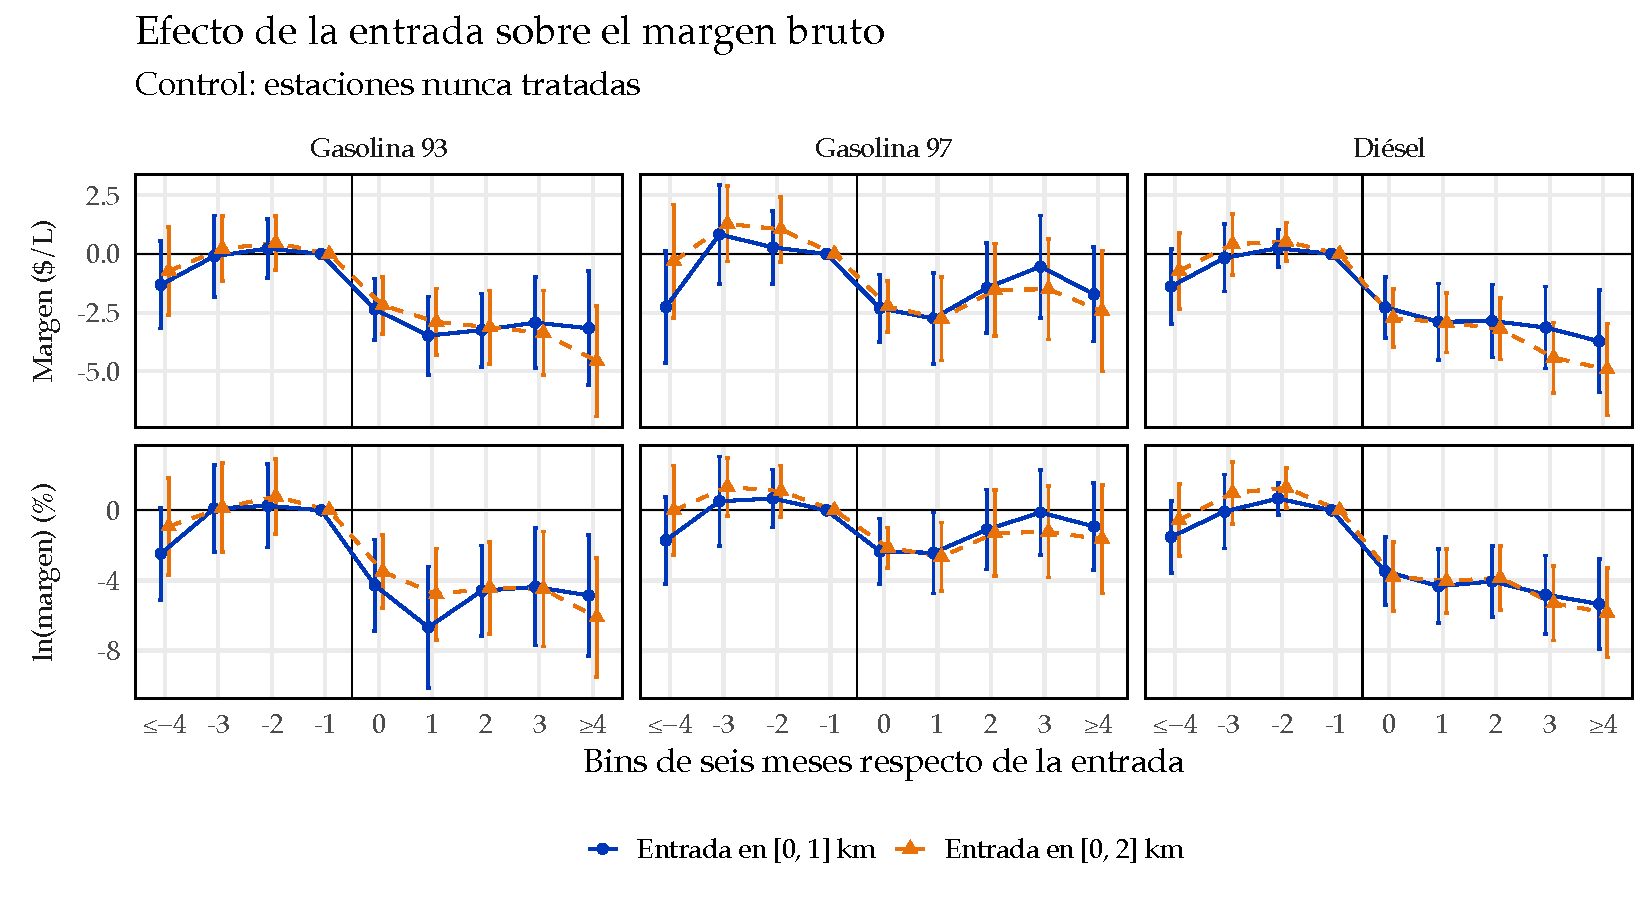
\includegraphics[width=\textwidth]{formato_fischer.pdf}
\caption{Efecto de la entrada sobre el margen bruto, por combustible}
\label{fig:ff}
\end{figure}

En el caso de la gasolina de 97 octanos se exhibe un efecto sistemáticamente menor y menos preciso, a un kilómetro no alcanza significancia convencional en ninguna de las dos unidades, y solo la logra al ampliar el radio a dos. La lectura que se desprende de esto es que a diferencia de la gasolina de 93 octanos la 97 es el combustible premium del mercado. Representa apenas el $3{,}3\%$ de las ventas nacionales de combustibles líquidos frente al $16\%$ de la 93 \parencite{FNE2025informe}, y sus consumidores plausiblemente presentan una demanda menos elástica al precio. Si la demanda que enfrenta la incumbente en ese producto es menos sensible, la llegada de un competidor genera menos presión para ajustarlo. El resultado es entonces informativo, pero conviene no apoyar en él ninguna conclusión que los otros dos combustibles no sostengan por sí solos.

La \Cref{hip:distancia} predice que el efecto decrece con la distancia entre la entrante y la incumbente y se anula a partir de un umbral. La
\Cref{fig:atenuacion} lo contrasta asignando cada estación al anillo de un kilómetro correspondiente a su primera entrada cercana y estimando el efecto por anillo.

\subsubsection{Atenuación por distancia}

\begin{figure}[H]
\centering
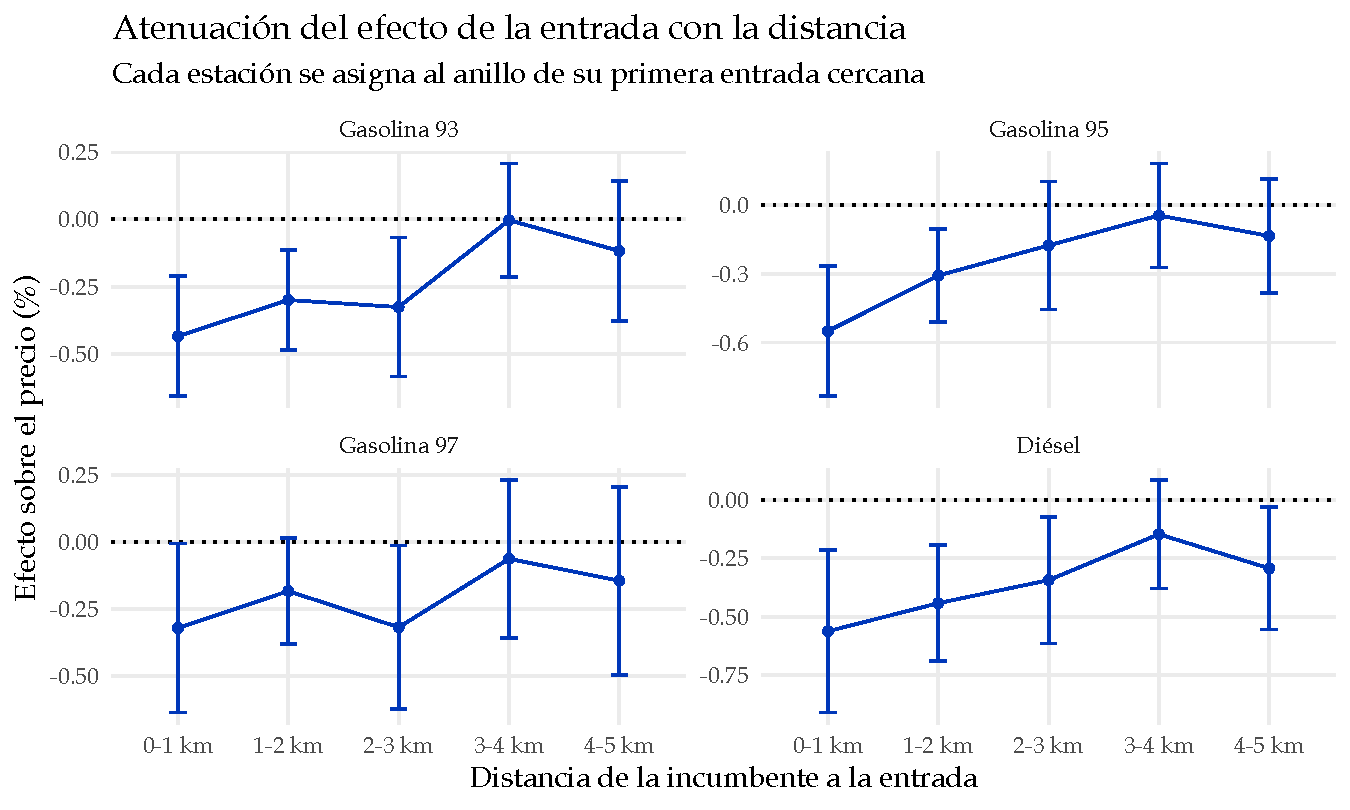
\includegraphics[width=\textwidth]{atenuacion_distancia.pdf}
\caption{Atenuación del efecto de la entrada con la distancia}
\label{fig:atenuacion}
\end{figure}

El perfil decae desde el anillo más cercano y deja de ser distinguible de cero entre los tres y los cuatro kilómetros. Por un lado, el resultado valida la predicción del modelo: como se explica en el Anexo~\ref{anexo:modelo}, lo que el perfil recupera es la proporción de incumbentes para las cuales la entrante cae dentro del radio en que la sustitución es efectiva, proporción que se agota a la distancia en que ya casi ninguna estación comparte mercado con la entrante. El umbral así estimado coincide con la delimitación de mercado geográfico que la \textcite{FNE2021informe} emplea en sus investigaciones. Por otro, es informativo a la hora de decidir utilizar o no controles dentro de los anillos entre 3 a 5km. Si el efecto sigue vivo a dos o tres kilómetros, el anillo de control necesariamente contiene estaciones parcialmente tratadas, lo que explica
por qué su estimación atenúa.

\subsubsection{Heterogeneidad según el margen previo}

\textcite{KOH2022} plantean que la respuesta a la competencia depende del margen con que la incumbente operaba antes de la entrada, una estación con márgenes holgados puede bajar precios, mientras que una que ya opera con márgenes estrechos carece de espacio para hacerlo y responde por otras vías, como reducir su probabilidad de seguir operando. Los autores no pueden contrastar esta hipótesis directamente, ya que no observan el precio mayorista y, por lo tanto, tampoco los márgenes de las estaciones, deben aproximarlos distinguiendo entre áreas metropolitanas y no metropolitanas, limitación que ellos mismos reconocen.

La disponibilidad del MEPCO permite contrastarla de manera directa. La \Cref{hip:margen} formula la misma predicción a partir de la \Cref{prop:margen}, donde el margen previo es una transformación exacta del número de competidoras efectivas de la incumbente. Para contrastarla hace falta una medida del margen con que cada estación operaba antes de la entrada, y esa medida debe cumplir dos condiciones.

La primera es que sea comparable entre estaciones que enfrentan costos y
mercados distintos. Se construye entonces como la \emph{posición relativa} de la
estación dentro de la distribución de precios de su propia comuna en cada mes.
Dentro de una comuna y un mes el costo mayorista es idéntico para todas las
estaciones y el margen porcentual es estrictamente creciente en el precio, de
modo que el orden de los precios es exactamente el orden de los márgenes. La
posición así definida es además adimensional, lo que permite promediarla entre
combustibles.

La segunda es que no esté construida sobre la misma variable que el resultado.
La medida es entonces un \emph{promedio ponderado} de la posición de la estación
en cada combustible, con ponderadores iguales a la participación relativa de cada
uno dentro de los cuatro combustibles analizados —$19{,}6\%$ la gasolina de 93
octanos, $11{,}9\%$ la de 95, $4{,}0\%$ la de 97 y $64{,}4\%$ el diésel,
calculados a partir de las ventas nacionales de 2017 que reporta
\textcite{FNE2025informe}— y \emph{excluyendo el combustible que se analiza en
cada caso}.\footnote{Los cuatro combustibles analizados concentran el $81{,}5\%$
de las ventas nacionales de combustibles líquidos, de modo que los ponderadores
son las participaciones informadas por la FNE renormalizadas sobre ese total.} Al estimar el efecto sobre el precio del diésel, por ejemplo, el
moderador se construye solo con las tres gasolinas.

La exclusión no es un refinamiento menor. El precio observado de una estación
tiene un componente persistente, que es el que interesa, y uno transitorio. Si
el moderador incluyera el propio combustible, el tercil superior quedaría
poblado en parte por estaciones que simplemente recibieron perturbaciones
positivas en la ventana previa, y esas perturbaciones revierten: el grupo alto
caería después con o sin entrada. Excluir el combustible analizado elimina ese
canal. El Anexo~\ref{anexo:moderador} compara esta definición con dos
alternativas más simples y cuantifica cuánto del contraste proviene de él.

Finalmente, la posición se mide siempre como el promedio sobre la ventana previa
a la entrada y nunca de manera contemporánea, ya que una medición posterior
sería un resultado del tratamiento y no una característica previa de la
estación.

\begin{table}[H]
\centering
\caption{Efecto de la entrada según el margen previo de la incumbente}
\label{tab:het}
\tabla{tab_het_rank}
\end{table}

La \Cref{tab:het} y la \Cref{fig:het} confirman la predicción. El efecto sobre
las estaciones del tercil superior de su comuna duplica o triplica al de las
restantes en los cinco resultados, y la fila de diferencia —que proviene de
reparametrizar el mismo modelo, de modo que su error estándar es el del
contraste y no el de una comparación visual de intervalos— es significativa al
$1\%$ en el precio del diésel y en su margen, y al $10\%$ en el precio de la
gasolina de 95 octanos. En los demás combustibles el contraste mantiene el signo
y una magnitud comparable sin alcanzar significancia convencional, de modo que en
ellos el resultado debe leerse como indicativo. Las trayectorias previas de ambos
grupos son planas, lo que descarta que el resultado sea reversión a la media.

\begin{figure}[H]
\centering
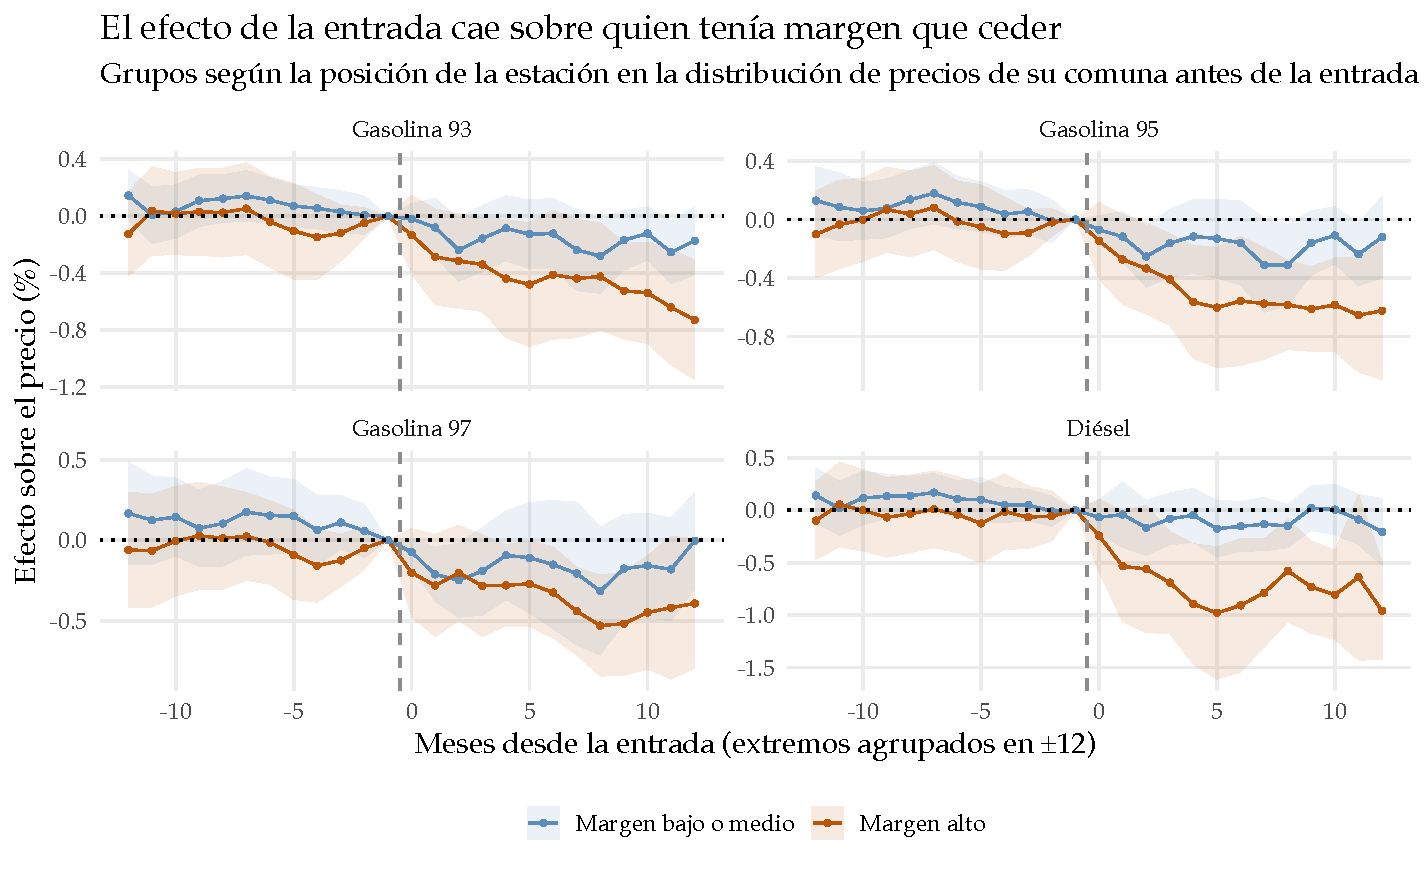
\includegraphics[width=\textwidth]{het_rank_precio.pdf}
\caption{Efecto de la entrada según el margen previo de la incumbente}
\label{fig:het}
\end{figure}

El resultado tiene una lectura que va más allá de la heterogeneidad. Lo que disciplina el precio no es la mera presencia de competidores, sino el margen que la incumbente venía capturando, que es la medida de su poder de mercado local. Es la misma conclusión a la que llega \textcite{BRESNAHAN1991} por otra vía: al inferir la conducta competitiva desde la relación entre número de firmas y tamaño del mercado en mercados locales aislados, encuentra que casi toda la variación ocurre con la entrada de la segunda o la tercera firma y que, una vez que el mercado tiene entre tres y cinco, la siguiente entrante apenas la altera. El efecto de una entrada no es constante, depende de cuán concentrado estaba el mercado que la recibe.

\subsection{Validez del supuesto de identificación}

El supuesto que sostiene el diseño no es que la entrada sea exógena, sino que lo sea el momento en que se materializa, condicional en los efectos fijos de \eqref{eq:es}. Esta subsección reúne la evidencia sobre esa afirmación. Los contrastes de tendencias previas, que son la verificación indirecta habitual, se presentan en el Anexo~\ref{anexo:control} junto con la comparación de grupos de control.

Conviene delimitar la afirmación antes de someterla a prueba, porque la mitad de las objeciones habituales apuntan a algo que el diseño no necesita. Como las cadenas eligen deliberadamente dónde instalarse, resulta inverosímil que la ubicación sea independiente de las condiciones del mercado local. La teoría lo anticipa desde el origen mismo de este marco: \textcite{HOTELLING1929} muestra que la competencia espacial genera un incentivo a instalarse cerca del rival y no lejos de él, y la evidencia estructural para este mismo mercado confirma que entrar y salir son decisiones dinámicas que responden a la rentabilidad esperada del mercado local y al marco regulatorio de precios que lo rige \parencite{HOUDE2005}. Los datos de este trabajo son consistentes con ambas cosas: el $72{,}6\%$ de las entradas ocurre teniendo al menos una estación vecina dentro de 2 kilómetros. Lo que se supone, entonces, no es que la ubicación sea exógena, sino que, condicional en el efecto fijo de estación y en los efectos de tiempo, la fecha precisa de apertura no responde a la evolución de los precios de las incumbentes.

Esta separación tiene un fundamento institucional en el caso chileno. La decisión de instalar una estación es endógena, pero entre esa decisión y la apertura media un rezago largo, variable y de naturaleza administrativa: adquisición o arriendo del terreno, permiso de edificación, exigencias del plan regulador comunal, autorización de la Superintendencia de Electricidad y Combustibles y recepción de obras. La \textcite{FNE2021informe} documenta que la escasez de terrenos aptos, precisamente por las exigencias de los planos reguladores en las zonas urbanas más saturadas, constituye la principal barrera a la entrada del mercado. Es ese rezago el que hace que el momento de apertura sea, desde la perspectiva de la incumbente, un evento cuya fecha no está ligada a su propia conducta de precios.

La \Cref{tab:escalera} estima \eqref{eq:did} sobre la misma muestra y con el mismo regresor, variando únicamente los efectos fijos. La comparación es la de la tabla 6 de \textcite{ARCIDIACONO2020}.

\begin{table}[H]
\centering
\caption{Efecto estimado según los efectos fijos incluidos}
\label{tab:escalera}
\tabla{tab_fe_ladder}
\end{table}

La especificación de sección cruzada arroja un efecto cercano al triple del que entrega la especificación preferida. Esa brecha es la medida de cuánto de la asociación bruta entre entrada y precios bajos proviene de dónde eligen instalarse las entrantes, y no de lo que su entrada provoca. El efecto fijo de estación es el que la elimina.



\section{Conclusiones}

Esta investigación tuvo el objetivo de cuantificar la reacción competitiva de EDS incumbentes frente a la presencia de nuevos competidores en el mercado chileno observando el comportamiento en precios de sus distintos productos. Bajo metodologías estándar en la literatura relacionada y aproximaciones del márgen de venta se pudo cuantificar la magnitud de la respuesta y caracterízarla. Se encontró que la entrada de un competidor dentro de 2 kilómetros reduce el margen de venta alrededor del $5\%$ en la gasolina 93 y diesel, con efectos no identificables y/o nulos en la gasolina 97. Estimaciones complementarias soportan ideas clave en la literatrura, tales como la atenuación del efecto dada la distancia y  que la respuesta competitiva depende de los márgenes ex-ante al condicionar la respuesta factible. 

El marco teórico que motivó las proposiciones se mantuvo firme frente a las pruebas empíricas. El modelo de \textcite{SALOP1979}, empleado en su formulación original y sin adaptaciones, funcionó bien para describir un mercado cuyo bien es homogéneo, precios altamente visibles y competencia espacial. Las tres hipótesis contrastadas se desprenden de sus resultados de equilibrio, y las tres encuentran respaldo en los datos.

Los resultados se conectan de manera directa con tres definiciones que la Fiscalía Nacional Económica emplea en su labor de fiscalización de este mercado. En primer lugar, la delimitación del mercado relevante geográfico, la \textcite{FNE2021informe} ha trabajado en la práctica con radios de tres a cinco kilómetros. El criterio que la autoridad viene aplicando por analogía y jurisprudencia tiene, entonces, respaldo empírico, y el extremo inferior del rango de tres kilómetros resulta el más apropiado para el análisis de operaciones de concentración.

En segundo lugar, el costo de las barreras a la entrada. La misma Fiscalía documenta que la escasez de terrenos aptos, derivada de las exigencias de los planos reguladores en las zonas urbanas más saturadas, constituye la principal barrera a la entrada de este mercado. Cada entrada que no ocurre son aproximadamente cuatro puntos porcentuales de margen que las incumbentes de ese mercado local retienen de manera indefinida. El resultado sugiere que la regulación de uso de suelo, tiene efectos de competencia mensurables sobre los precios que enfrentan los consumidores.

En tercer lugar, y de manera más específica, la heterogeneidad orienta dónde concentrar el escrutinio. Si la respuesta competitiva se concentra en las estaciones que venían capturando márgenes altos en relación con su entorno, la posición relativa del margen es un indicador observable y de bajo costo para identificar mercados locales donde la entrada tendría mayor efecto disciplinador.

Tres limitaciones conviene reconocer. La primera es que no se dispone de una medida de demanda local a la escala del mercado relevante que permita descartar que la entrada coincida con un aumento de la demanda del sector. La segunda es que el MEPCO es una referencia nacional y no regional, de modo que cualquier diferencial de costo geográfico queda dentro del margen medido. La tercera es que no se observan cantidades vendidas por estación, lo que impide estimar el efecto sobre ingresos y, con ello, evaluar el canal de salida que documentan \textcite{ARCIDIACONO2020} y \textcite{KOH2022}.






\newpage

\printbibliography

\newpage

\appendix

\section{El modelo de competencia espacial: desarrollo y fuentes}
\label{anexo:modelo}

Este anexo desarrolla el modelo que la \Cref{prop:margen} y el
\Cref{cor:entrada} resumen en el cuerpo. Ninguno de los resultados es original:
todos provienen de \textcite{SALOP1979} y el anexo indica, para cada uno, la
ecuación y la página del artículo de las que se obtiene.\footnote{El artículo se
publicó en el \emph{Bell Journal of Economics}, vol.~10, n.º~1, pp.~141--156.
Conviene advertir que Salop no enuncia sus resultados como proposiciones ni
teoremas numerados, sino como ecuaciones dentro del desarrollo del texto; la
numeración empleada aquí y en el cuerpo es propia de este trabajo y sirve
únicamente para referirse a ellos.} El propósito del anexo es doble: dejar
trazable el origen de cada expresión y reunir las limitaciones del marco, que en
el cuerpo se omiten por brevedad.

\subsection{El problema del consumidor}

El mercado local se representa por una circunferencia de perímetro unitario
sobre la que se distribuyen uniformemente $L$ consumidores, cada uno con demanda
unitaria e inelástica por combustible. Operan $n$ estaciones equiespaciadas, de
modo que la distancia entre dos contiguas es $1/n$. Un consumidor localizado a
distancia $x$ de la estación $i$ obtiene un excedente
\begin{equation}
    U_i(x) = v - p_i - c\,x ,
    \label{eq:anexo-utilidad}
\end{equation}
donde $v$ es el precio de reserva efectivo —la valoración del combustible neta
del excedente que otorga el bien externo, ecuación (4) de
\textcite[142]{SALOP1979}— y $c>0$ el costo de desplazamiento por unidad de
distancia. El consumidor compra una unidad en la estación que le entregue el
mayor excedente, siempre que este sea no negativo.

La formulación \eqref{eq:anexo-utilidad} recoge dos rasgos del mercado chileno
descritos en el cuerpo. Primero, la homogeneidad del producto: dos EDS que cobran
el mismo precio son indiferentes para el consumidor, y solo la distancia las
separa. Segundo, la observabilidad de precios, que permite tratar al consumidor
como informado sobre $p_i$ en todo el mercado local.

\subsection{Las tres regiones de la curva de demanda}

\textcite[143--145]{SALOP1979} distingue tres regiones según cuán agresivo sea el
precio de la estación representativa en relación con sus vecinas, ilustradas en
su Figura~1.

\paragraph{Región de monopolio local.} Si el precio de $i$ es suficientemente
alto, la estación solo atrae a los consumidores para quienes el excedente
\eqref{eq:anexo-utilidad} es no negativo, sin llegar a disputar clientes a sus
vecinas. El consumidor marginal se ubica a una distancia $\hat{x}=(v-p_i)/c$, de
modo que la demanda es
\begin{equation}
    q^{m} = \frac{2L}{c}\,(v - p_i) ,
    \label{eq:anexo-qm}
\end{equation}
que es la ecuación (6) de \textcite[143]{SALOP1979}. En esta región la estación
compite contra el bien externo —no comprar, o abastecerse fuera del mercado
local— y no contra sus vecinas.

\paragraph{Región competitiva.} Si el precio es lo bastante bajo como para que
los mercados potenciales de estaciones contiguas se traslapen, el consumidor
marginal ya no es aquel indiferente entre comprar y no comprar, sino aquel
indiferente entre dos estaciones. La demanda es entonces
\begin{equation}
    q^{c} = \frac{L}{c}\left(\bar{p} + \frac{c}{n} - p_i\right) ,
    \label{eq:anexo-qc}
\end{equation}
donde $\bar{p}$ es el precio de las vecinas; es la ecuación (9) de
\textcite[144]{SALOP1979}. Esta es la región relevante para el análisis, pues es
la que corresponde a los mercados urbanos donde ocurre la mayoría de las
entradas.

\paragraph{Región supracompetitiva.} Con precios aún menores la estación captura
la totalidad del mercado de su vecina, situación que aparece bajo la ecuación
(12) de \textcite[145]{SALOP1979}. No se considera aquí, pues corresponde a
comportamientos predatorios ajenos al fenómeno estudiado.

Derivando \eqref{eq:anexo-qm} y \eqref{eq:anexo-qc} se obtienen las pendientes de
la demanda en cada región, $-2L/c$ y $-L/c$ respectivamente, que son las
ecuaciones (10) y (11) de \textcite[144]{SALOP1979}. La distinción entre las dos
primeras regiones tiene una consecuencia empírica directa, que la
\Cref{hip:distancia} recoge y que la \Cref{prop:monopolio} formaliza más abajo.

\subsection{El margen de equilibrio}

Cada estación elige $p_i$ tomando como dados los precios de sus vecinas y
maximizando $(p_i - m)\,q_i - F$, donde $m$ es el costo marginal, común a todas
las estaciones por el argumento del MEPCO expuesto en el cuerpo, y $F$ el costo
fijo de operación del sitio. Imponiendo la condición de primer orden —ecuación
(13) de \textcite[147]{SALOP1979}— sobre la pendiente de la demanda competitiva
se obtiene el resultado de la \Cref{prop:margen},
\begin{equation}
    p = m + \frac{c}{n} ,
    \qquad\text{esto es}\qquad
    \mu = \frac{c}{n} ,
    \label{eq:anexo-margen}
\end{equation}
que es la ecuación (18) de \textcite[147]{SALOP1979}. El margen es proporcional
al costo de desplazamiento e inversamente proporcional al número de competidoras;
equivalentemente, y puesto que las estaciones están equiespaciadas, es
proporcional a la distancia $1/n$ que separa a la estación de sus vecinas. Esta
doble lectura es la que permite que el margen opere en la estrategia empírica
como medida de aislamiento espacial.

\subsection{El umbral: monopolio local}

\begin{proposicion}[Monopolio local]
\label{prop:monopolio}
Si los mercados de estaciones contiguas no se traslapan, la estación resuelve un
problema de monopolio frente al bien externo y su precio óptimo es
\begin{equation}
    p^{m} = \frac{v + m}{2} ,
    \label{eq:monopolio}
\end{equation}
que no depende de $n$ ni de la ubicación de las vecinas.
\end{proposicion}

Se obtiene maximizando el beneficio de monopolio de la ecuación (28) de
\textcite[151]{SALOP1979}, cuya solución es la cantidad $q^{m}=(L/c)(v-m)$ de su
ecuación (29), y sustituyéndola en la demanda de monopolio
\eqref{eq:anexo-qm}, que invertida es $p = v - (c/2L)\,q$. Es el único de los
resultados empleados que Salop no escribe en términos de precio, pues su interés
en esa sección está en las condiciones de rentabilidad y no en el precio de
monopolio.

La proposición es la que dota al modelo de un umbral. Mientras no haya traslape
de mercados, la estructura del mercado local es irrelevante para el precio, de
modo que una entrada lo bastante lejana deja a la incumbente exactamente donde
estaba. El modelo no predice, a nivel de estación, una atenuación asintótica sino
la existencia de un umbral.

\subsection{Entrada libre}

\begin{proposicion}[Entrada libre]
\label{prop:libre}
Bajo libre entrada, el número de estaciones y el margen de equilibrio son
\begin{equation}
    n^{*} = \sqrt{cL/F} ,
    \qquad
    \mu^{*} = \frac{c}{n^{*}} = \sqrt{cF/L} ,
    \label{eq:entrada-libre}
\end{equation}
de modo que el número de estaciones es creciente en la densidad de consumidores
del mercado local y decreciente en el costo fijo de instalación, y el margen se
mueve en sentido inverso.
\end{proposicion}

Son las ecuaciones (19), p.~147, y (22), p.~148, de \textcite{SALOP1979}, que el
autor obtiene de la condición de beneficio nulo (14) evaluada en el equilibrio
competitivo; la expresión para $n^{*}$ se repite como su ecuación (23). Mercados
más densos sostienen más estaciones y márgenes menores.

Conviene señalar que estas dos predicciones —la \Cref{prop:margen} y la
\Cref{prop:libre}— ya han sido contrastadas de manera directa en este mismo
mercado. \textcite{CLEMENZGUGLER2006} toman el modelo de \textcite{SALOP1979}
como marco teórico explícito y derivan de él dos hipótesis: que las estaciones se
ubican más densamente donde la densidad de población es mayor, y que el precio de
equilibrio es menor mientras mayor sea la densidad de estaciones. Encuentran
apoyo para ambas en el mercado minorista austríaco. La densidad de población
explica más del $95\%$ de la variación entre distritos en la densidad de
estaciones, y el coeficiente de la densidad de estaciones sobre el precio tiene el
signo predicho y es significativo al $5\%$ o mejor en todas sus especificaciones;
estimar el sistema como ecuaciones simultáneas no altera sus conclusiones y
sugiere que la causalidad corre desde la densidad hacia el precio, que es la
dirección que este trabajo explota usando una entrada como fuente de variación.

Dos detalles de ese trabajo importan aquí. El primero es que predicen que la
densidad de estaciones crece de manera \emph{cóncava} en la densidad de
población, porque la mayor proximidad reduce el precio de equilibrio y con ello
el beneficio que sostiene a cada sitio. Es exactamente la raíz cuadrada de
\eqref{eq:entrada-libre}. El segundo es la lectura de competencia que le dan a su
segunda hipótesis: la ausencia de una relación negativa entre densidad y precio
sería señal de que las estaciones coordinan sus precios en lugar de competir. Que
en este trabajo una entrada reduzca el margen de las incumbentes es, bajo esa
lectura, evidencia de que la competencia local opera y no está suprimida por
coordinación.

Conviene además situar el ejercicio en la tradición que inaugura
\textcite{BRESNAHAN1991}, que infiere la intensidad de la competencia a partir de
la relación entre el número de firmas y el tamaño del mercado en mercados locales
geográficamente aislados. Su hallazgo central es que la conducta competitiva
cambia rápido con las primeras entradas y casi deja de cambiar después: en
mercados con cinco firmas o menos, casi toda la variación ocurre con la entrada
de la segunda o la tercera, y una vez que el mercado tiene entre tres y cinco
firmas la siguiente entrante casi no altera la conducta. Es el patrón que
\eqref{eq:anexo-efecto} predice, puesto que $c/(n(n+1))$ decrece rápidamente en
$n$, y es el mismo mecanismo que sostiene la \Cref{hip:margen}: la incumbente que
más pierde ante una entrada cercana es la que operaba con pocas competidoras y,
por lo tanto, con márgenes altos.

\subsection{El efecto de una entrada y las tres hipótesis}

El \Cref{cor:entrada} es la estática comparativa directa de
\eqref{eq:anexo-margen} respecto de $n$, tratando el número de competidoras como
un parámetro de corto plazo,
\begin{equation}
    \Delta\mu = \frac{c}{n+1} - \frac{c}{n} = -\,\frac{c}{n(n+1)} \;<\; 0 .
    \label{eq:anexo-efecto}
\end{equation}
No aparece como tal en \textcite{SALOP1979}, cuya sección 4 (pp.~148--149)
desarrolla las estáticas comparativas respecto de los parámetros
$\{F, m, v, c, L\}$ y no respecto del número de firmas, que en su análisis de
largo plazo es endógeno. La diferencia es de horizonte y no de contenido: la
\Cref{prop:libre} describe hacia dónde converge el mercado en el largo plazo,
mientras que \eqref{eq:anexo-efecto} describe el ajuste de precios de las
incumbentes ante un cambio en $n$ que ellas toman como dado, que es el objeto de
este trabajo.

Dado que $m$ está determinado por una referencia nacional y la entrada es un
evento local, el costo marginal no se altera y la caída del margen se traslada
uno a uno al precio, $\Delta p = \Delta\mu$. Esta equivalencia es la que permite
contrastar el modelo tanto con precios como con márgenes, y es consecuencia
directa del carácter nacional del MEPCO.

\paragraph{Sobre el nivel (\Cref{hip:nivel}).} El signo de
\eqref{eq:anexo-efecto} es inequívoco para cualquier entrada que aumente el
número de competidoras efectivas de la incumbente. El efecto es además
permanente, pues opera sobre el equilibrio del mercado local y no sobre una
desviación transitoria respecto de él.

\paragraph{Sobre la distancia (\Cref{hip:distancia}).} Por la
\Cref{prop:monopolio}, una entrada que no genere traslape de mercados deja a la
incumbente frente al bien externo, donde su precio óptimo \eqref{eq:monopolio} es
independiente de la estructura del mercado local, y el efecto es exactamente
nulo. Conviene precisar qué predice el modelo y qué no. Para una estación dada la
predicción es discontinua: la entrante cuenta en $n_i$ o no cuenta, y el efecto es
$-c/(n_i(n_i+1))$ o cero. Lo que se estima empíricamente, en cambio, es el efecto
promedio por anillo de distancia sobre estaciones cuyo radio de mercado difiere.
Como la proporción de incumbentes para las cuales la entrante cae dentro del
radio decrece con la distancia, el promedio de umbrales heterogéneos genera un
perfil que decae de manera suave y se anula más allá de cierta distancia. Es ese
perfil, y no una atenuación asintótica a nivel de estación, lo que la
\Cref{hip:distancia} afirma y lo que la \Cref{fig:atenuacion} contrasta.

\paragraph{Sobre el margen previo (\Cref{hip:margen}).} Por
\eqref{eq:anexo-margen}, el margen es un estadístico suficiente del aislamiento
espacial de la estación: $\mu$ es alto precisamente cuando las competidoras son
pocas y están lejos. Invirtiendo \eqref{eq:anexo-margen} como $n = c/\mu$ y
sustituyendo en \eqref{eq:anexo-efecto}, el efecto de una entrada se expresa
directamente en función del margen previo,
\begin{equation}
    |\Delta\mu| = \frac{\mu^{2}}{c + \mu} ,
    \qquad
    \frac{\partial\,|\Delta\mu|}{\partial\mu}
    = \frac{\mu\,(2c + \mu)}{(c + \mu)^{2}} \;>\; 0 ,
    \label{eq:het}
\end{equation}
de modo que una incumbente con margen previo elevado es una incumbente aislada y
es, por lo tanto, la que más pierde ante una entrada cercana. La predicción vale
además en términos relativos, que es la escala en que se estiman los resultados
sobre el precio en logaritmo: $|\Delta\mu|/\mu = \mu/(c+\mu)$ es también
creciente en $\mu$.

Vale la pena notar que la formulación en términos de $\mu$ y no del número de
competidoras dentro de un radio fijo no es una elección de conveniencia. El
conteo $n_i(r) = \#\{j : \mathrm{dist}(i,j) \le r\}$ se construye sobre un radio
$r$ igual para todas las estaciones, mientras que el $n_i$ del modelo es el
número de competidoras dentro del radio propio de cada mercado local, que no se
observa. Por \eqref{eq:anexo-margen}, en cambio, $\mu$ es una transformación
exacta de ese $n_i$. El margen es, en este modelo, el estadístico suficiente del
poder de mercado local, y el conteo a radio fijo apenas una aproximación gruesa.

\subsection{Limitaciones del marco}

Tres limitaciones conviene declarar. La primera es que el equilibrio de
\textcite{SALOP1979} predice un margen común a todas las estaciones que enfrentan
el mismo $n$, mientras que los datos muestran dispersión de precios persistente
dentro de mercados muy estrechos. Leer la circunferencia como el mercado local de
cada estación, y no como una unidad administrativa, acomoda parte de esa
dispersión, pues estaciones de una misma comuna enfrentan distinto $n_i$; pero no
toda. La literatura atribuye el resto a fricciones informativas del lado del
consumidor \parencite{FISCHER2025}, un canal que este modelo no incorpora.

La segunda es que el equiespaciamiento es un supuesto de conveniencia y no un
rasgo del mercado chileno. Su función es hacer que $1/n$ sea a la vez el
espaciamiento y el inverso del número de competidoras, de modo que ambas lecturas
de \eqref{eq:anexo-margen} coincidan. Con espaciamiento desigual las magnitudes
cambian, pero no el signo ni el ordenamiento en que descansan las tres hipótesis.

La tercera es que la \Cref{prop:libre} describe la entrada como una respuesta a
la densidad del mercado local, es decir, como una decisión endógena respecto de
dónde instalarse. La estrategia de identificación desarrollada en el cuerpo no
requiere negar esa endogeneidad sino únicamente que el momento preciso en que la
entrada se materializa sea exógeno desde la perspectiva de la incumbente.


\section{Construcción del panel de precios}
\label{anexo:datos}

Este anexo documenta las decisiones de construcción resumidas en la subsección
de Datos. Se detallan aquí porque condicionan lo que el diseño puede
identificar, pero su discusión completa interrumpiría la lectura del cuerpo.

\subsection{Identidad de la estación física}

La unidad de análisis es la estación física y no el identificador
administrativo de la CNE, porque un mismo local puede aparecer en el registro
bajo más de un código. Se detectaron dos situaciones, de naturaleza distinta.

\paragraph{Sucesión.} Un identificador nuevo comienza a reportar en el mismo
punto donde otro dejó de hacerlo. El criterio aplicado es que la primera fecha
del identificador entrante sea igual o posterior a la última del saliente y que
ambos disten menos de cincuenta metros. Corresponde típicamente a un cambio de
operador del mismo local. Si no se fusionaran, el cambio de operador se
contaría como una salida seguida de una entrada, es decir, se fabricaría un
evento de tratamiento donde no hubo ninguna alteración de la estructura
competitiva local.

\paragraph{Duplicación.} Los archivos del régimen antiguo llevan, para 31
estaciones, un segundo identificador formado agregando el sufijo \texttt{a} al
código base. La evidencia de que se trata del mismo local es concluyente: en
los 31 casos el código base también está presente en el registro, en los 31
casos ambos identificadores coexisten desde el inicio de la serie —no se
suceden— y los 31 dejan de reportarse cuando la CNE migra al formato actual,
que incorpora una columna de modalidad de atención. Es decir, lo que el régimen
antiguo llevaba como dos registros separados, el nuevo lo consolida en un solo
registro con dos modalidades.

La duplicación es más dañina que la sucesión para este trabajo. Dos registros
del mismo local aparecen en el panel como dos estaciones distintas separadas
por una distancia nula, de modo que cada una cuenta a la otra como competidora
inmediata. Esto no solo infla el número de estaciones del mercado, sino que
contamina precisamente la variable —el número de competidores en un radio
dado— que el diseño usa para delimitar los mercados locales.

Ambas situaciones se resuelven encadenando los identificadores hasta una raíz
común, que define la estación física. Tras la fusión, el registro contiene
2.030 estaciones físicas.

\subsection{Frecuencia del panel}

El panel se construye a frecuencia semanal sobre la grilla de jueves del MEPCO
y de ahí se colapsa a frecuencia mensual, tomando la última semana de cada mes.

La elección de la semana responde a dos hechos. El primero es la cadencia
efectiva de reporte: la mediana es de cincuenta observaciones por estación,
combustible y año, es decir, aproximadamente una por semana. El segundo es que
el precio mayorista con MEPCO se fija semanalmente y rige desde el jueves, de
modo que la semana es la unidad natural del costo.

Construir el panel a frecuencia diaria habría sido posible, pero cerca del
$85\%$ de sus celdas correspondería a un valor arrastrado desde el último
reporte, sin información adicional, y con observaciones perfectamente
correlacionadas dentro de cada semana. En la grilla semanal, en cambio, el
$81{,}1\%$ de las celdas corresponde a un precio efectivamente informado esa
semana.

\subsection{Arrastre y ventanas de actividad}

Dentro de cada estación y combustible el precio se arrastra hacia adelante
hasta un máximo de trece semanas, aproximadamente tres meses. El arrastre
refleja el hecho de que un precio no informado sigue vigente: la obligación
legal es informar cada variación, de modo que la ausencia de reporte significa
que el precio no cambió.

El tope cumple la función opuesta. Un vacío superior a trece semanas deja a la
estación fuera del panel durante esas semanas, de manera que un precio no se
arrastra a través de un período en que la estación no operaba o no reportaba.
Sin este tope, una estación cerrada durante un año seguiría figurando en el
panel con su último precio conocido, y sería contada como competidora activa de
sus vecinas.

\subsection{Márgenes}

El margen bruto se define como el precio de venta menos el precio mayorista con
MEPCO vigente esa semana, conforme a la \Cref{prop:margen}. Al ser el MEPCO una
referencia nacional fijada por regla, el costo se adjudica por combustible y
semana y no por estación.

La variable existe para el $82{,}4\%$ de las observaciones del panel. El resto
se reparte entre dos causas conocidas: la gasolina de 95 octanos, para la que no
se publica referencia MEPCO, y los meses anteriores a agosto de 2014, cuando el
mecanismo todavía no operaba. Ninguna de las dos introduce selección, ya que
ambas son ausencias por combustible y por período, no por estación.

Las series descriptivas de precio y margen del cuerpo excluyen los meses que el
panel no abarca de extremo a extremo. En la práctica esto descarta julio de
2026: el registro termina el día 12 de ese mes y el promedio queda construido
sobre dos semanas que además caen en medio de un traspaso inacabado, ya que el
precio mayorista había caído 95 pesos por litro el 18 de junio y el precio
minorista continuaba ajustándose. El margen promedio de ese mes es un artefacto
de truncamiento, no un resultado de mercado.

\subsection{Restricciones sobre la definición de entrada}

Una entrada se define como el primer mes en que una estación física aparece en
el registro. Sobre esa definición operan tres restricciones, que son las que
determinan qué eventos pueden usarse como tratamiento.

\paragraph{Censura por la izquierda.} Las estaciones presentes desde el inicio
de la serie no constituyen entradas: 1.548 de las 2.030 estaciones ya reportaban
en 2012 y su fecha de apertura es desconocida. Tratarlas como entrantes en enero
de 2012 fecharía como evento lo que es apenas el comienzo de la observación.

\paragraph{La cohorte de 2013.} Ese año se registran 79 entradas, contra veinte
a cincuenta en un año normal, y 43 de ellas corresponden a estaciones de bandera
blanca, cifra que no se repite en ningún otro año de la serie. Es el patrón de
una incorporación tardía al sistema de reporte —estaciones pequeñas que se
suman a Bencina en Línea cuando la plataforma ya está en marcha— y no el de una
ola de aperturas. Estos eventos se conservan para efectos de contaminación y de
corte de las ventanas, de modo que un incumbente expuesto a una de ellas no se
usa como si nada le hubiera ocurrido, pero nunca definen una cohorte de
tratamiento.

\paragraph{Solo la primera entrada.} De cada incumbente se considera únicamente
la primera entrada cercana, y las observaciones posteriores a una segunda se
descartan. El estimando corresponde así al efecto de una primera entrada y no a
una mezcla de efectos de primera y segunda, que no tienen por qué ser iguales:
el paso de un competidor a dos altera la estructura del mercado local de manera
distinta que el paso de dos a tres.

\subsection{Salidas y el quiebre de régimen de reporte}

El diseño empírico se construye exclusivamente sobre entradas, pero conviene
documentar por qué no se utilizan las salidas.

El cambio entre los archivos del régimen antiguo y los del actual deja una
cicatriz nítida: cien estaciones dejan de ser informadas en diciembre de 2022,
contra una o dos al año en todo el período posterior. Una parte de ese salto
corresponde a las duplicaciones ya descritas. El resto son, con alta
probabilidad, estaciones que habían dejado de actualizar sus precios en alguna
fecha anterior no observada y que sobrevivían en los archivos anuales con su
último precio conocido hasta que la migración las depuró.

La consecuencia es que la fecha de salida de esas estaciones no es
interpretable: lo único que se observa es el momento en que el sistema dejó de
listarlas, que no coincide con el momento en que dejaron de operar. Por eso las
tablas descriptivas reportan diciembre de 2022 en una categoría separada, en
lugar de diluirlo dentro de un total anual que sugeriría una ola de cierres que
no ocurrió.

Esta limitación no se traslada al diseño. La primera aparición de una estación
en el registro sí es una fecha interpretable, porque una estación que no existe
no puede informar precios. Un ejercicio de verificación confirma que las
entradas no arrastran el problema: de las 482 entradas identificadas, ninguna
tiene una estación que haya dejado de reportar dentro de los cincuenta metros
en los dieciocho meses previos, y solo siete la tienen dentro de doscientos
metros.

\subsection{Reemplazo de estaciones salientes}

Una precisión sobre cómo debe leerse la información de reemplazo. Dado que la
fusión de identificadores descrita más arriba ya une a una estación con su
sucesora en el mismo sitio, un reemplazo en el mismo local no puede aparecer en
los datos como una salida: aparece como continuidad de la misma estación
física. La pregunta que sí tiene contenido empírico es, entonces, si el mercado
local se repuso, y se responde verificando si abrió alguna estación a menos de
quinientos metros dentro de los veinticuatro meses siguientes al cierre. La
respuesta es que casi nunca ocurre, lo que resulta consistente con las barreras
a la entrada que documenta la \textcite{FNE2021informe}.


\section{Elección del grupo de comparación}
\label{anexo:control}

Este anexo desarrolla la comparación entre las tres definiciones posibles del
grupo de control que la subsección de Identificación resume. La conclusión es
que las nunca tratadas —el criterio de \textcite{FISCHER2025}— no es superior en
todos los frentes, sino la única definición que no reprueba de manera marcada en
ninguno.

Las tres definiciones son: el \emph{anillo}, formado por las incumbentes
situadas entre 2 y 5 kilómetros del evento; el grupo \emph{lejano}, formado por
las estaciones que nunca estuvieron a menos de 5 kilómetros de una entrada; y
las \emph{nunca tratadas}, que es la unión de las dos anteriores y equivale al
conjunto de estaciones que nunca reciben una entrada dentro del radio de
tratamiento. Las tres se estiman sobre la misma muestra de tratadas y con la
misma especificación, de modo que la única diferencia es contra quién se las
compara.

Conviene tener presente desde el inicio que las nunca tratadas no son un cuarto
grupo independiente sino la suma de los otros dos. Cualquier característica en
que aparezcan como intermedias lo son por construcción, al ser un promedio
ponderado de un grupo próximo a las tratadas y otro alejado, y no por una
propiedad sustantiva propia.

\subsection{Magnitud y precisión}

La \Cref{tab:control} del cuerpo muestra que las tres definiciones entregan
estimaciones muy próximas entre sí. Ese hecho es, por sí mismo, el resultado más
importante de este anexo: la conclusión no depende de la elección, de modo que
esta no es un grado de libertad del que dependa el signo o el orden de magnitud
del efecto.

Donde sí difieren es en precisión. Las nunca tratadas más que duplican el tamaño
del anillo y superan al grupo lejano, y en consecuencia entregan el error
estándar más bajo en los cuatro combustibles cuando el resultado es el precio, y
en dos de los tres cuando es el margen. La \Cref{tab:balance} reporta el número
de estaciones de cada grupo junto con sus características promedio antes del
tratamiento.

\begin{table}[H]
\centering
\caption{Balance de covariables y tamaño de cada grupo de comparación}
\label{tab:balance}
\tabla{tab_balance_control}
\end{table}

\subsection{Comparabilidad y contaminación}

La \Cref{tab:balance} deja ver por qué ninguno de los dos subconjuntos domina al
otro.

El anillo es el más parecido a las tratadas en cuatro de las cinco dimensiones
observadas. Comparte con ellas el entorno urbano y opera en mercados de densidad
comparable: 6,2 competidores dentro de 2 kilómetros contra 8,9 de las tratadas,
mientras que las lejanas apenas alcanzan 2,1. La brecha de margen es de 9,9
pesos por litro, frente a 38,8 del grupo lejano. Pero el anillo es también el
grupo contaminado: el ejercicio de atenuación por distancia del cuerpo muestra
que el efecto de la entrada sigue siendo distinto de cero en la banda de 2 a 3
kilómetros, que es precisamente su borde interior. Un control parcialmente
tratado atenúa la estimación hacia cero.

El grupo lejano es la imagen inversa. Está limpio de contaminación por
construcción, ya que ninguna de sus estaciones estuvo jamás a menos de 5
kilómetros de una entrada, pero es el peor balanceado en todas las dimensiones
salvo una. Sus mercados son estructuralmente más ralos, su margen promedio
supera en un $55\%$ al de las tratadas, y solo el $9\%$ de sus estaciones está
en la Región Metropolitana contra el $30\%$ de las tratadas. Usarlo en exclusiva
expone la estimación a que una diferencia de tendencia entre mercados urbanos y
rurales se confunda con el efecto de la entrada.

La excepción es la composición regional, y ahí el orden se invierte. El anillo se
desvía veintidós puntos por encima de las tratadas en participación
metropolitana y el grupo lejano veinte puntos por debajo, de modo que al unirlos
ambos sesgos se cancelan y las nunca tratadas quedan a un punto de las tratadas.
Es la ilustración más clara del punto anterior: la ventaja es aritmética, no
sustantiva, pero no por ello menos real para el diseño.

En las demás dimensiones las nunca tratadas heredan una parte de cada problema y
ninguna en su forma extrema. Conviene notar que la contaminación que hereda del
anillo opera en una dirección conocida: atenúa el efecto hacia cero, de modo que
la estimación resultante debe leerse como una cota inferior en magnitud y no
como un valor que podría estar inflado.

\subsection{Tendencias previas}

La \Cref{tab:pretend} reporta, para cada grupo y combustible, dos contrastes
sobre el período previo a la entrada. El primero es el test conjunto de que todos
los coeficientes anteriores a $\tau = -1$ son nulos. El segundo es la pendiente
de la trayectoria previa, junto con la deriva que esa pendiente acumularía en
doce meses expresada como fracción del efecto estimado.

\begin{table}[H]
\centering
\caption{Contrastes de tendencias previas por grupo de comparación}
\label{tab:pretend}
\tabla{tab_pretend_control}
\end{table}

La distinción entre ambos contrastes no es un tecnicismo. El test conjunto
evalúa la hipótesis nula contra alternativas arbitrarias y tiene, por esa misma
razón, poca potencia frente a una deriva lineal suave, que es justamente la
forma que importaría. El contraste de pendiente es el que tiene potencia contra
esa alternativa, y la razón entre la deriva acumulada y el efecto estimado es la
que permite juzgar si una pendiente estadísticamente indistinguible de cero es,
aun así, lo bastante grande como para explicar una fracción relevante del
resultado.

Bajo el contraste de pendiente ninguna de las tres definiciones se aproxima a la
significancia convencional: los valores $p$ van de $0{,}58$ a $0{,}97$. Las
derivas acumuladas, en cambio, no son despreciables en todos los casos, y su
lectura exige atender al signo. En once de las doce combinaciones de grupo y
combustible la deriva previa es de signo contrario al efecto estimado, es decir,
los precios de las tratadas venían subiendo respecto de los controles antes de
la entrada. Una pre-tendencia de ese signo no puede generar el resultado: opera
en contra de encontrarlo, y hace que la estimación sea conservadora.

La magnitud sí distingue entre grupos. En el grupo lejano la deriva alcanza el
$71\%$ del efecto estimado en la gasolina de 95 octanos y el $48\%$ en la de 97,
mientras que en las nunca tratadas no supera el $38\%$ y en el anillo el $41\%$.
Es un argumento adicional, y del mismo signo que los anteriores, contra usar el
grupo lejano en exclusiva.

\subsection{Síntesis}

La \Cref{fig:comparacion} superpone las tres trayectorias estimadas sobre la
misma muestra de tratadas. Se distinguen apenas entre sí, tanto antes como
después de la entrada.

\begin{figure}[H]
\centering
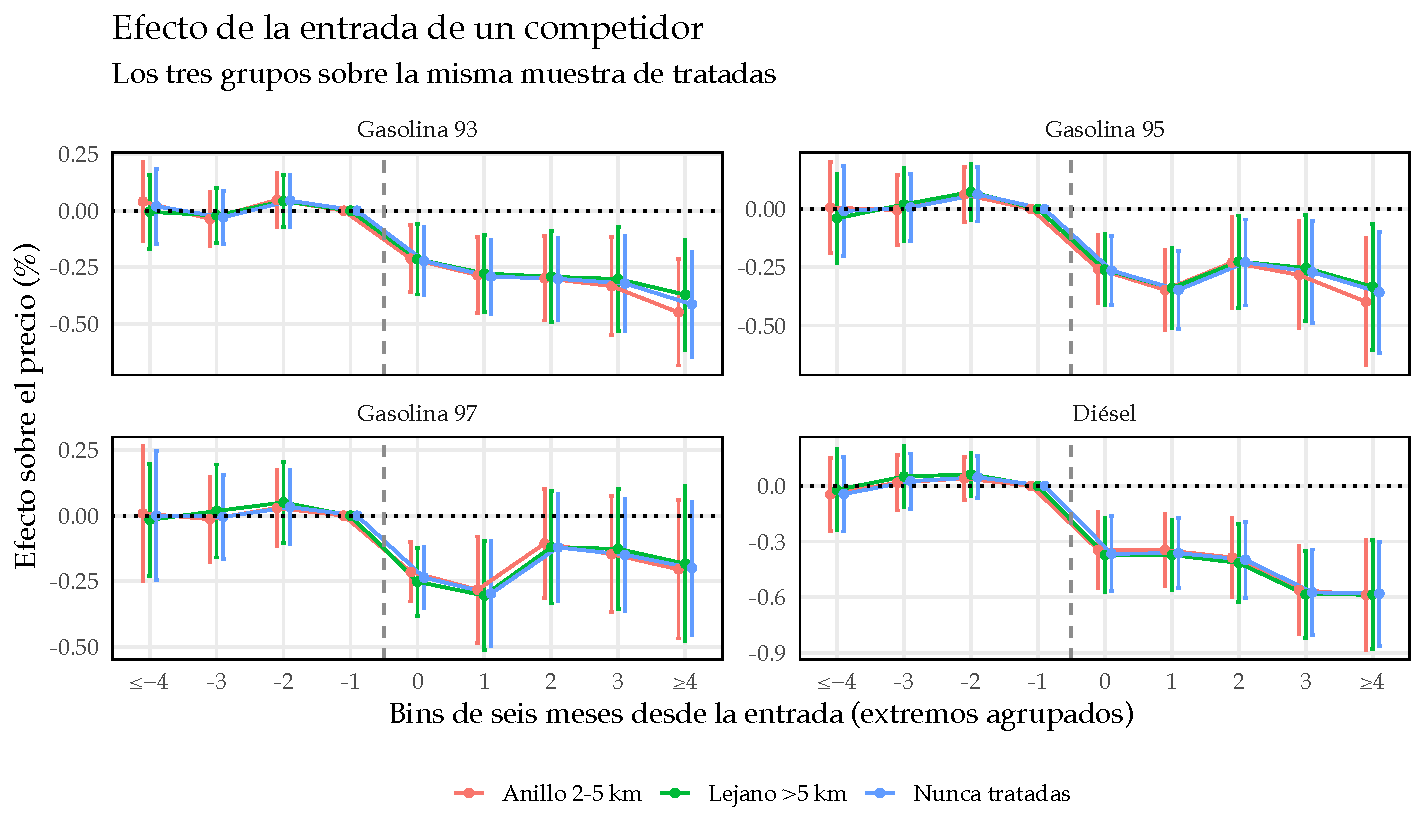
\includegraphics[width=\textwidth]{es_control_comparacion.pdf}
\caption{Estudio de eventos bajo las tres definiciones del grupo de comparación}
\label{fig:comparacion}
\end{figure}

Los criterios se resumen así. En precisión gana el conjunto de las nunca
tratadas; en comparabilidad gana el anillo, salvo en composición regional; en
ausencia de contaminación gana el grupo lejano. Las nunca tratadas es la única
alternativa que no queda en último lugar en ninguno de los tres, y es además el
criterio que emplea \textcite{FISCHER2025} en un diseño de las mismas
características, lo que hace que la elección tenga precedente y no dependa del
juicio del autor.


\section{Robustez del estimador y persistencia del tratamiento}
\label{anexo:robustez}

\subsection{Estimador escalonado}

El diseño tiene veinticinco cohortes semestrales de entrada repartidas sobre
doce años. En ese contexto el estimador de diferencias en diferencias con
efectos fijos bidireccionales es un promedio ponderado de comparaciones entre
cohortes en el que unidades ya tratadas actúan como control de unidades tratadas
más tarde, y las ponderaciones pueden ser negativas cuando el efecto del
tratamiento varía entre cohortes \parencite{SUNABRAHAM2021}. Es el problema que
la literatura reciente ha documentado para diseños escalonados.

La \Cref{tab:sunab} reestima el efecto promedio con el estimador ponderado por
interacción de \textcite{SUNABRAHAM2021}, sobre la misma muestra y con los
mismos efectos fijos, de modo que la única diferencia entre columnas es el
estimador.

\begin{table}[H]
\centering
\caption{Efecto promedio de la entrada: Sun y Abraham frente a TWFE}
\label{tab:sunab}
\tabla{tab_sunab}
\end{table}

Las dos columnas son prácticamente idénticas en los cuatro combustibles, y las
diferencias entre ellas son muy inferiores a los errores estándar. La
\Cref{fig:sunab} muestra que la coincidencia se extiende a toda la trayectoria
del estudio de eventos y no solo al promedio.

\begin{figure}[H]
\centering
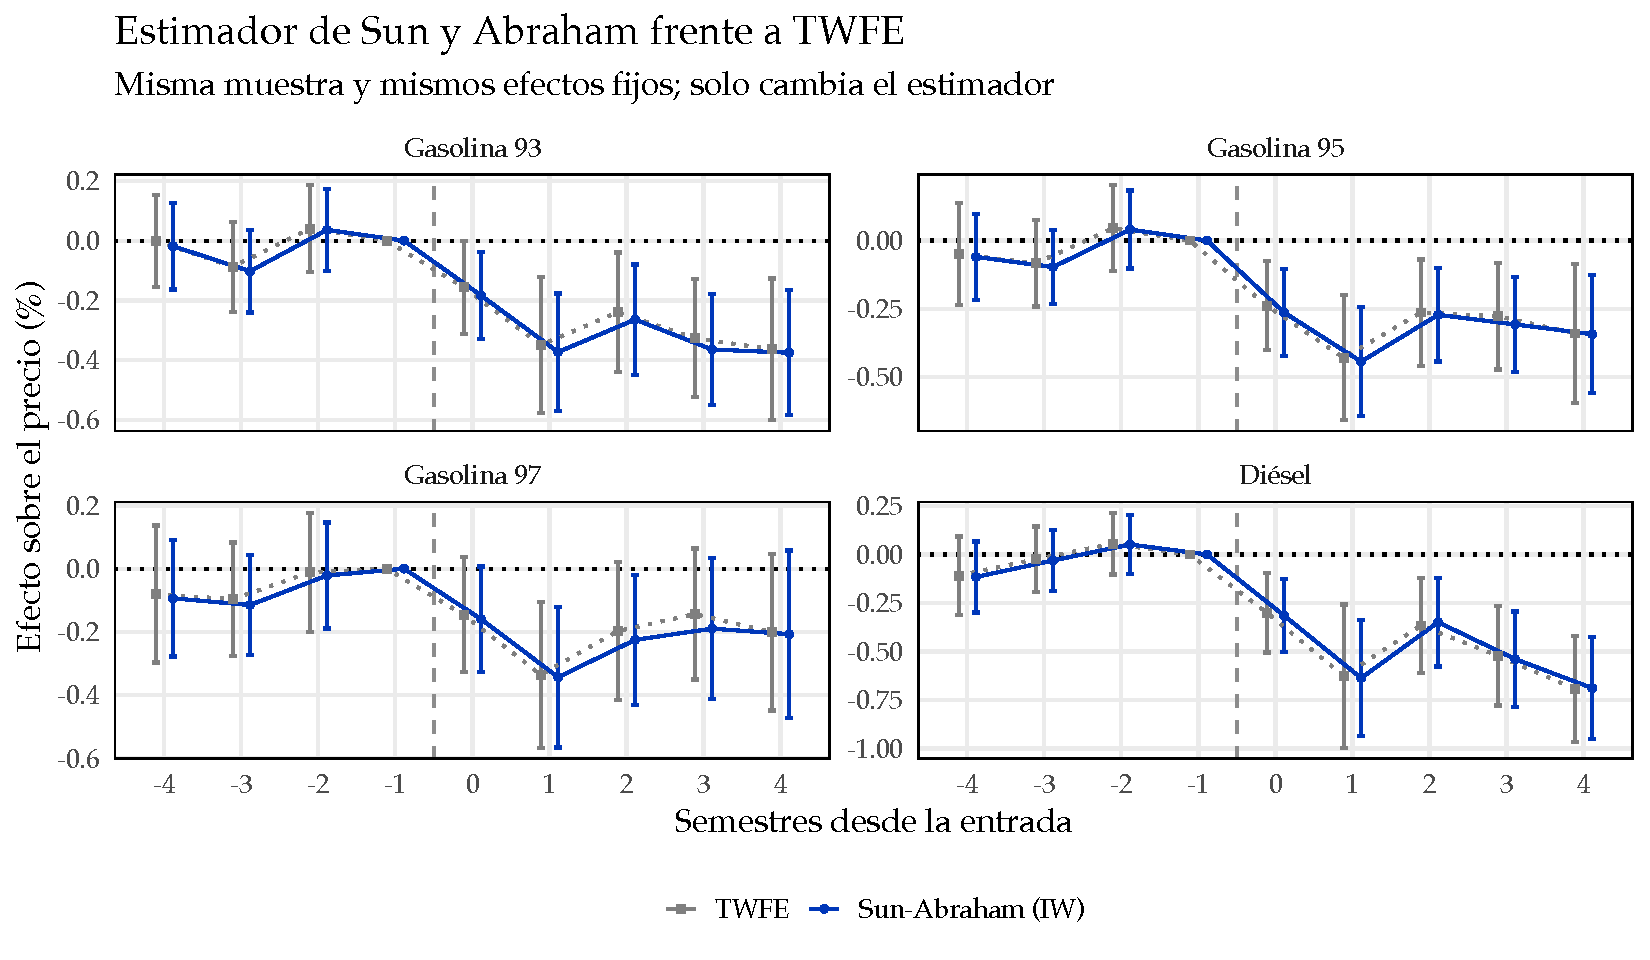
\includegraphics[width=\textwidth]{sunab_vs_twfe.pdf}
\caption{Trayectoria estimada por Sun y Abraham frente a TWFE}
\label{fig:sunab}
\end{figure}

El resultado no es sorprendente y tiene una explicación conocida: el sesgo por
heterogeneidad de efectos entre cohortes se vuelve pequeño cuando la mayoría de
las unidades de comparación nunca son tratadas, ya que en ese caso las
comparaciones problemáticas —entre una cohorte tratada y otra ya tratada—
reciben poco peso. Este diseño está en esa situación, con cerca de seiscientas
estaciones nunca tratadas frente a algo más de setecientas tratadas.

\subsection{Persistencia del tratamiento}

El diseño trata a la entrada como un aumento discreto y duradero del número de
competidores del mercado local. La \Cref{fig:persistencia} verifica ambos
supuestos con dos estudios de eventos que replican la figura 2 de
\textcite{FISCHER2025}, usando como resultado el propio conteo de estaciones y
no el precio.

\begin{figure}[H]
\centering
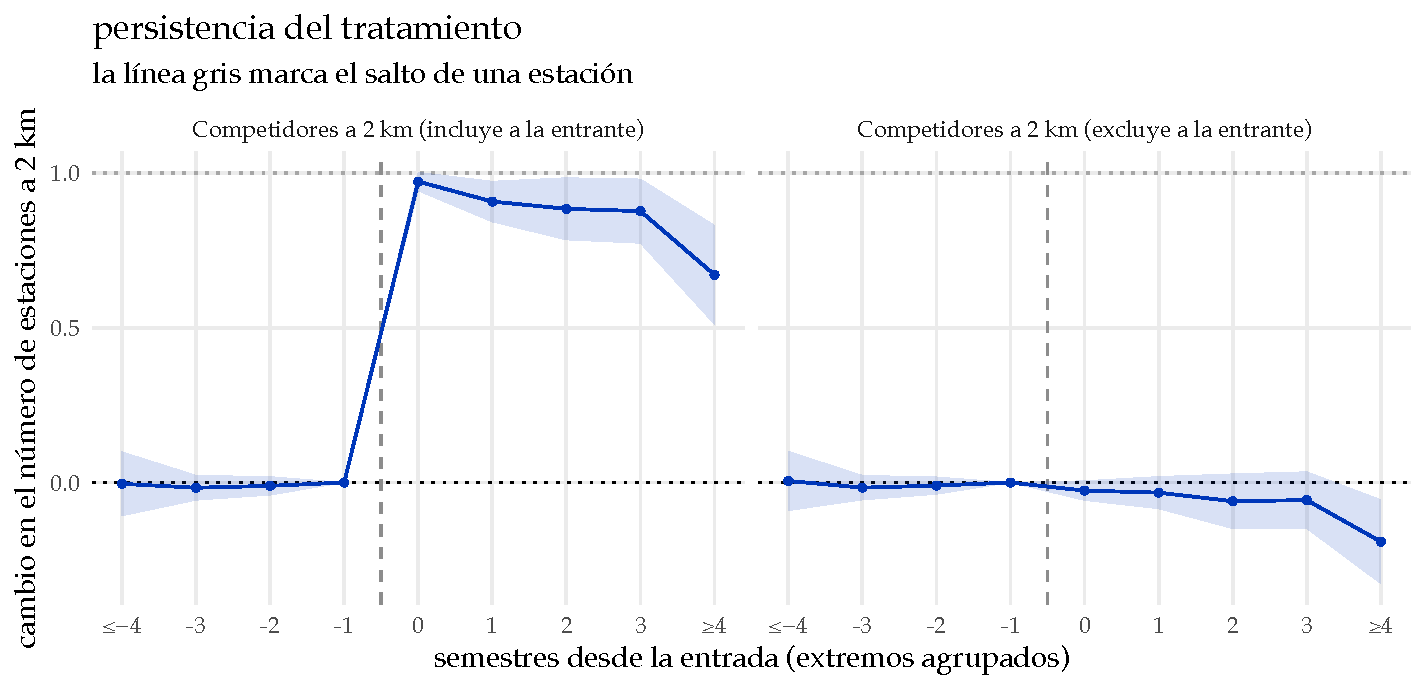
\includegraphics[width=\textwidth]{persistencia.pdf}
\caption{Efecto de la entrada sobre el número de estaciones del mercado local}
\label{fig:persistencia}
\end{figure}

El panel izquierdo cuenta todas las estaciones activas dentro de 2 kilómetros
de la incumbente, incluida la entrante. El conteo salta prácticamente en una
unidad en el semestre de la entrada y se mantiene elevado durante los semestres
siguientes: el tratamiento ocurre y perdura. El salto no es exactamente igual a
uno porque no todas las estaciones informan precios cada mes, de modo que el
conteo mide presencia efectiva en el registro y no capacidad instalada.

El panel derecho es el sustantivo. Cuenta solo las estaciones que ya operaban
antes de la entrada, es decir, excluye a la entrante. Esa serie permanece plana:
la entrada no desplaza a las incumbentes del mercado, al menos dentro del
horizonte analizado. La verificación importa porque, de haber desplazamiento, el
efecto estimado sobre los precios sería en parte un efecto de composición
—cambiaría el conjunto de estaciones sobre el que se promedia— y no una
respuesta competitiva de las estaciones que permanecen.

Se observa una leve caída de ambas series en el último bin, que agrupa todo lo
ocurrido más allá de dos años. Es consistente con la atrición natural del
registro a horizontes largos y no altera la lectura de los primeros cuatro
semestres, que es el horizonte sobre el que se interpreta el efecto.


\section{Efecto sobre la distribución de precios del mercado local}
\label{anexo:mercado}

El cuerpo estima el efecto de la entrada sobre el precio de cada incumbente. Ese
ejercicio responde cuánto baja el precio, pero no dónde del mercado local se
produce la baja, y esa segunda pregunta es la que determina quién se beneficia.
Si la entrada arrastra hacia abajo tanto a la estación más cara como a la más
barata, la ganancia se reparte entre todos los consumidores; si comprime el
mercado desde abajo, se concentra en quienes comparan precios antes de comprar.

\subsection{Diseño}

La unidad de observación cambia: es el mercado y no la estación. Un mercado se
define como el círculo de radio dado alrededor de una incumbente focal, y las
variables de resultado son el precio máximo, el promedio y el mínimo entre todas
las estaciones activas dentro de él. Se estima la misma especificación de
\eqref{eq:did}, con efecto fijo de mercado en lugar de estación.

Dos decisiones merecen mención. La primera es que el precio de la entrante
\emph{sí} entra en los agregados desde el mes en que abre. \textcite{FISCHER2025}
excluyen a las entrantes del análisis a nivel de estación, pero advierten que sus
precios importan para la elección del consumidor y las incorporan justamente en
este ejercicio; el criterio se replica aquí. Omitirlas sesgaría el resultado
precisamente donde interesa, ya que en Chile la entrante típica es de bandera
blanca y tiende a fijar precios bajos.

La segunda es que se exige al mercado tener al menos dos estaciones, medidas
\emph{antes} del tratamiento. Si la restricción se aplicara con el conteo
contemporáneo, seleccionaría sobre la propia entrada, que es lo que altera ese
conteo.

Se excluye de este ejercicio el efecto fijo de marca por año que sí lleva la
especificación principal: el resultado pertenece al mercado y no a la estación
focal, de modo que la marca de esta última no es el control apropiado.

\subsection{Resultados}

La \Cref{fig:mercado93} y la \Cref{fig:mercadodi} presentan los tres agregados
para la gasolina de 93 octanos y para el diésel, en las dos definiciones de
mercado.

\begin{figure}[H]
\centering
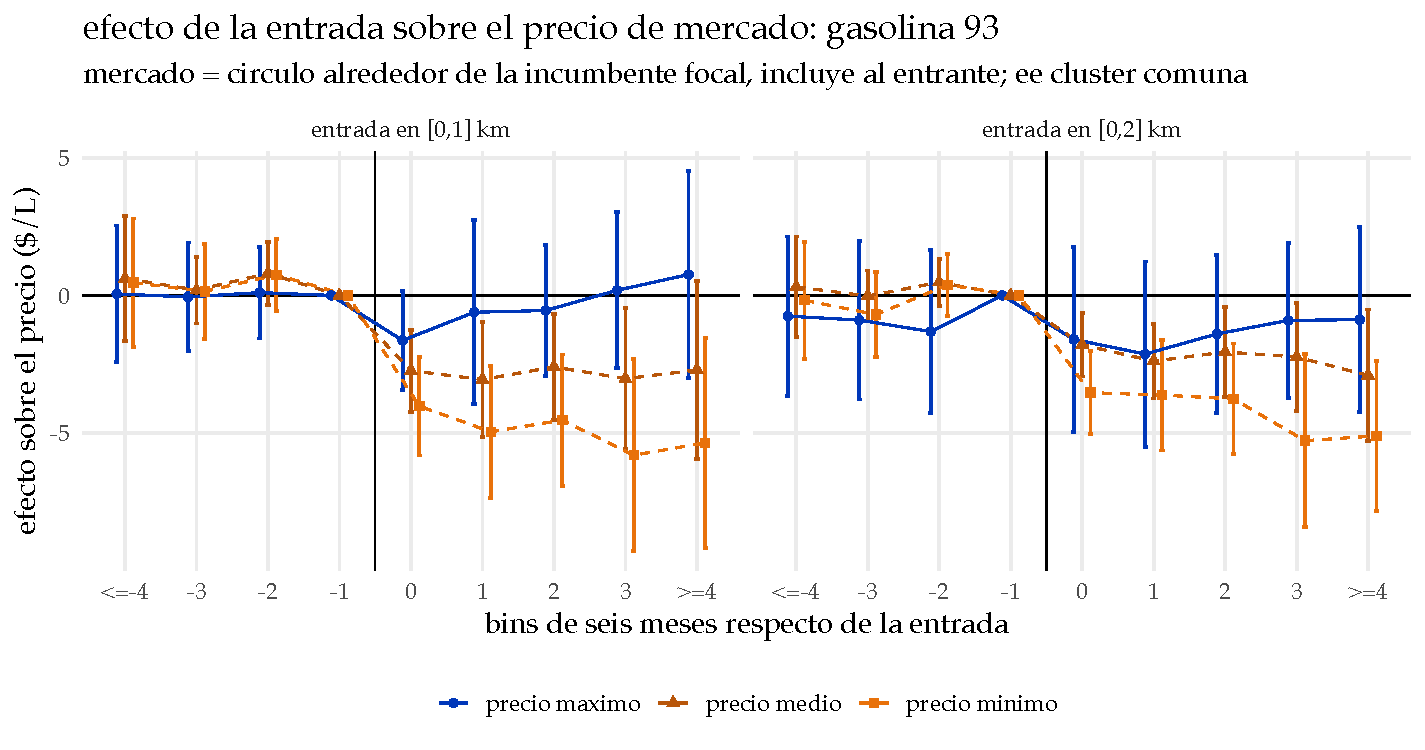
\includegraphics[width=\textwidth]{mercado_max_media_min_p93.pdf}
\caption{Efecto de la entrada sobre el precio máximo, medio y mínimo del mercado: gasolina de 93 octanos}
\label{fig:mercado93}
\end{figure}

\begin{figure}[H]
\centering
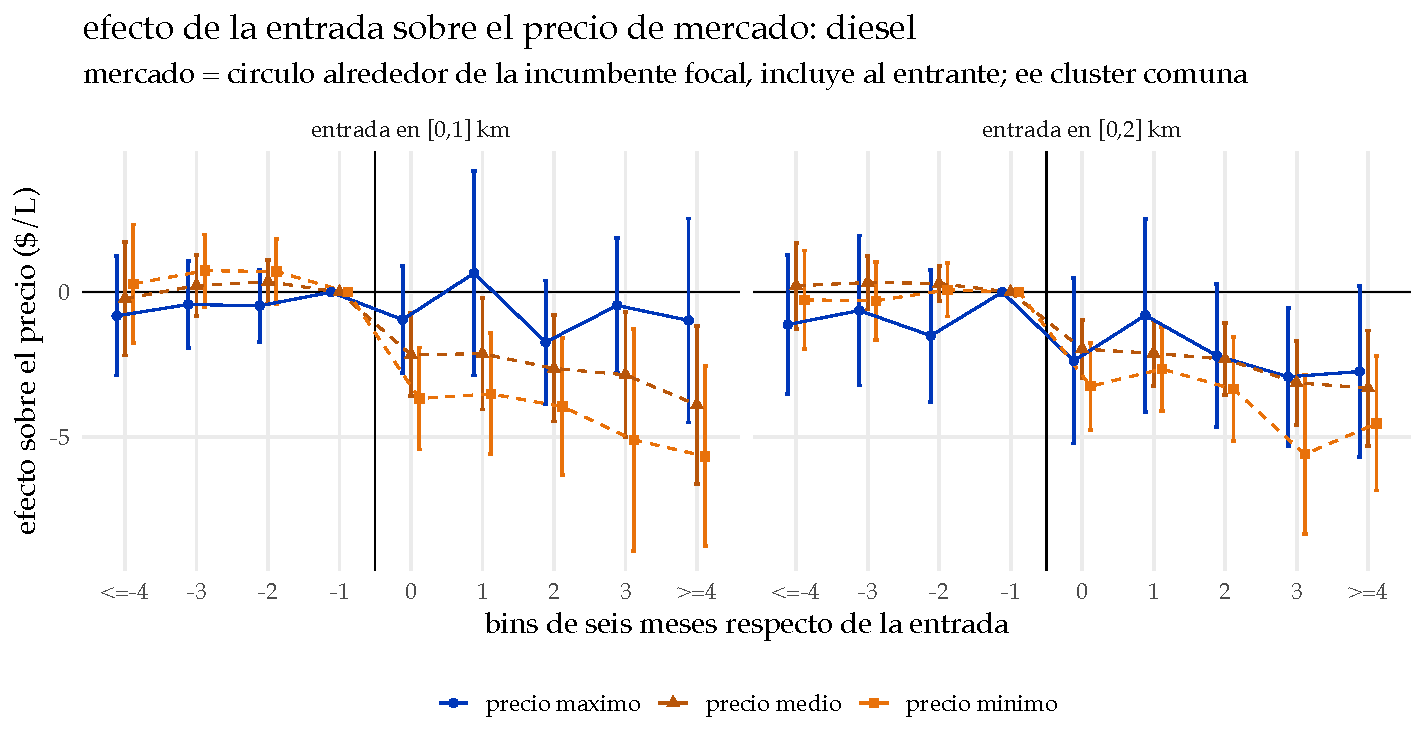
\includegraphics[width=\textwidth]{mercado_max_media_min_pdi.pdf}
\caption{Efecto de la entrada sobre el precio máximo, medio y mínimo del mercado: diésel}
\label{fig:mercadodi}
\end{figure}

El patrón es inequívoco y se repite en ambos combustibles: la entrada comprime
la distribución de precios del mercado desde abajo. Dentro de un kilómetro, el
precio mínimo cae 5,5 pesos por litro en la gasolina de 93 octanos y 5,4 en el
diésel, mientras que el máximo no se mueve de manera distinguible de cero. El
promedio, que es el objeto que estima la especificación principal, se ubica entre
ambos.

La lectura económica es directa. La estación que ya era la más barata del mercado
responde a la entrada bajando aún más, mientras que la más cara no reacciona.
Esto es consistente con un mercado en que conviven consumidores con distinto
grado de información o distinto costo de búsqueda: quien compara precios se
beneficia de una caída varias veces mayor que quien compra en la estación más
próxima sin comparar. Es también coherente con los resultados de heterogeneidad
del cuerpo, aunque se trate de objetos distintos —allí los cuantiles son de la
distribución de márgenes entre estaciones, aquí de los estadísticos de orden
dentro de cada mercado local— y con lo que encuentran \textcite{FISCHER2025} para
Alemania.

Conviene señalar una limitación de precisión. El error estándar del efecto sobre
el precio máximo es grande, de modo que la afirmación de que el máximo no
responde es un no rechazo y no una estimación precisa de cero. Establecer con
propiedad que la entrada desplaza la distribución en el sentido de dominancia
estocástica de primer orden exigiría los contrastes formales sobre la
distribución completa que se discuten en las extensiones de las conclusiones, y
que la muestra chilena no permite sostener.


\section{Construcción del margen previo y definiciones alternativas}
\label{anexo:moderador}

El contraste de heterogeneidad del cuerpo divide a las incumbentes según el
margen con que operaban antes de la entrada. Este anexo detalla cómo se
construye esa medida y por qué se descartan dos definiciones más simples.

\subsection{Por qué una posición relativa y no el margen en niveles}

El objeto que interesa es el poder de mercado local de la estación, que la
\Cref{prop:margen} identifica con el margen de equilibrio $\mu_i = c\,\bar{d}_i$.
El margen en niveles, sin embargo, no es comparable entre estaciones: depende
del combustible, del momento y del mercado en que la estación opera.

La medida empleada es por eso la posición relativa de la estación dentro de la
distribución de precios de su propia comuna en cada mes. Dos propiedades la
hacen apropiada. La primera es que dentro de una comuna y un mes todas las
estaciones enfrentan el mismo costo mayorista, dado que el MEPCO es una
referencia nacional; como el margen porcentual $(p - m)/p$ es estrictamente
creciente en $p$ cuando $p > m > 0$, el orden de los precios coincide
exactamente con el orden de los márgenes. La posición relativa mide entonces el
margen sin necesidad de calcularlo. La segunda es que, al ser un percentil, es
adimensional, lo que permite promediarla entre combustibles cuyos niveles de
precio difieren.

Hay además una razón teórica para preferir la comparación \emph{dentro} de la
comuna. Por la \Cref{prop:margen}, el margen ordena estaciones por aislamiento
espacial solo si el costo de desplazamiento $c$ es común entre ellas. Ese
supuesto es insostenible entre Santiago y una ruta interurbana, pero razonable
dentro de una misma comuna. Comparar posiciones dentro de comuna, y no niveles
entre comunas, es lo que hace que la medida siga leyéndose como aislamiento.

Se exige que la comuna tenga al menos cuatro estaciones en el mes para que el
percentil signifique algo. La restricción tiene un costo: descarta el $23\%$ de
las estaciones de la muestra, con mayor incidencia entre los controles, de modo
que la muestra de este ejercicio es menor que la de la especificación principal.

\subsection{Ponderación entre combustibles}

Una estación vende cuatro combustibles y su poder de mercado no se expresa por
igual en todos. La medida agrega las cuatro posiciones con ponderadores iguales
a la participación de cada combustible en el volumen nacional de ventas que
reporta \textcite{FNE2025informe} para 2017, renormalizados de modo que sumen
uno: $19{,}6\%$ la gasolina de 93 octanos, $11{,}9\%$ la de 95, $4{,}0\%$ la de
97 y $64{,}4\%$ el diésel.

Ponderar por volumen y no por igual evita que la gasolina de 97 octanos, que es
apenas el $4\%$ del mercado, pese lo mismo que el diésel, que es casi dos
tercios. La contrapartida es que los ponderadores provienen de ventas
nacionales, que incluyen canales distintos del minorista —el diésel tiene usos
industriales y de generación eléctrica que no pasan por estaciones de
servicio—, de modo que probablemente sobrerrepresentan el diésel respecto de lo
que vende una estación típica. No existe una desagregación pública por canal que
permita corregirlo.

\subsection{Por qué se excluye el combustible analizado}

El precio observado de una estación puede descomponerse en un componente
persistente, que refleja su aislamiento y es el que interesa, y uno transitorio.
Al seleccionar el tercil superior se seleccionan estaciones que son caras por
ambas razones a la vez. Las que lo son por una perturbación transitoria
favorable revierten después, con entrada o sin ella, de modo que el grupo alto
exhibiría una caída posterior aunque el tratamiento no existiera. Es la forma
que adopta aquí la reversión a la media.

Dos rasgos del diseño la contienen. El primero es que la posición se promedia
sobre toda la ventana previa —cuarenta y ocho meses en la mediana— y no se
toma de un mes aislado, lo que reduce el peso del componente transitorio. El
segundo, y el decisivo, es que el moderador excluye el combustible que se está
analizando: al estimar el efecto sobre el precio del diésel, el moderador se
construye únicamente con las tres gasolinas. La perturbación transitoria que
afectó al diésel de esa estación en la ventana previa no participa entonces de
la clasificación.

Conviene ser preciso sobre el alcance de esta corrección. Elimina el canal en
que la clasificación y el resultado comparten literalmente la misma variable,
pero no aquel en que una perturbación común a la estación mueve todos sus
combustibles a la vez. La correlación entre las posiciones de la gasolina de 93
octanos y del diésel es de $0{,}59$ a nivel de estación y mes, de modo que queda
contaminación residual. La verificación que cierra el argumento es empírica y no
de diseño: las trayectorias previas de ambos grupos son planas, con valores $p$
entre $0{,}18$ y $0{,}92$, lo que es incompatible con una reversión que ya
estuviera en curso antes de la entrada.

\subsection{Comparación con definiciones alternativas}

La \Cref{tab:moderador} reporta la diferencia entre grupos bajo tres
definiciones del moderador, estimadas sobre la misma especificación: el rango del
propio combustible, que es la versión más simple; el compuesto ponderado que
incluye los cuatro combustibles; y el compuesto que excluye el analizado, que es
el utilizado.

\begin{table}[H]
\centering
\caption{Diferencia entre grupos según la definición del margen previo}
\label{tab:moderador}
\tabla{tab_het_moderador}
\end{table}

La comparación entrega tres lecciones.

Primero, agregar combustibles mejora la medida. El paso de la definición A a la
C aumenta la magnitud del contraste y reduce su error estándar en la gasolina de
95 octanos y en el diésel. Promediar cuatro posiciones atenúa el error de
medición del moderador, y una variable de partición menos ruidosa separa mejor a
los grupos.

Segundo, la brecha entre B y C cuantifica el canal mecánico. En el diésel, cuyo
ponderador propio es de $0{,}64$, la definición B arroja una diferencia de
$-0{,}686$ y la C una de $-0{,}562$: cerca de un quinto del contraste bajo B
proviene de incluir el propio combustible en el moderador. Adoptar B produciría
un resultado más nítido a costa de reintroducir justamente el sesgo que se busca
evitar.

Tercero, el caso de la gasolina de 97 octanos es ilustrativo. Bajo la definición
A, que usa su propio rango, el contraste es de $-0{,}357$ y significativo al
$5\%$; bajo la definición C cae a $-0{,}220$ y deja de serlo. La 97 es el
combustible de menor volumen y precio más volátil, es decir, aquel en que el
componente transitorio pesa más, y es por lo tanto donde la definición ingenua
produce el resultado más engañoso. Es la razón concreta por la que este trabajo
no la utiliza.


\end{document}